\chapter{Exemplo de Uso} \label{cap:estudodecaso}
Com o intuito de comparar o desenvolvimento de aplicações móveis utilizando a abordagem nativa e multiplataforma, 
foi realizado um estudo preliminar. Para isso, um aplicativo feito em iOS 
nativo foi recriado utilizando o \textit{framework} Ionic. A seguir, o aplicativo escolhido é detalhado em termos de funcionalidades e recursos utilizados. 

\section{Descrição do projeto selecionado} \label{sec:descricaodoprojeto}

Mini Farma é um aplicativo criado inicialmente para a plataforma iOS que serve para controle dos medicamentos que as 
pessoas possuem em casa em suas ``farmacinhas'' particulares.

\begin{figure}[h]
  \centering
    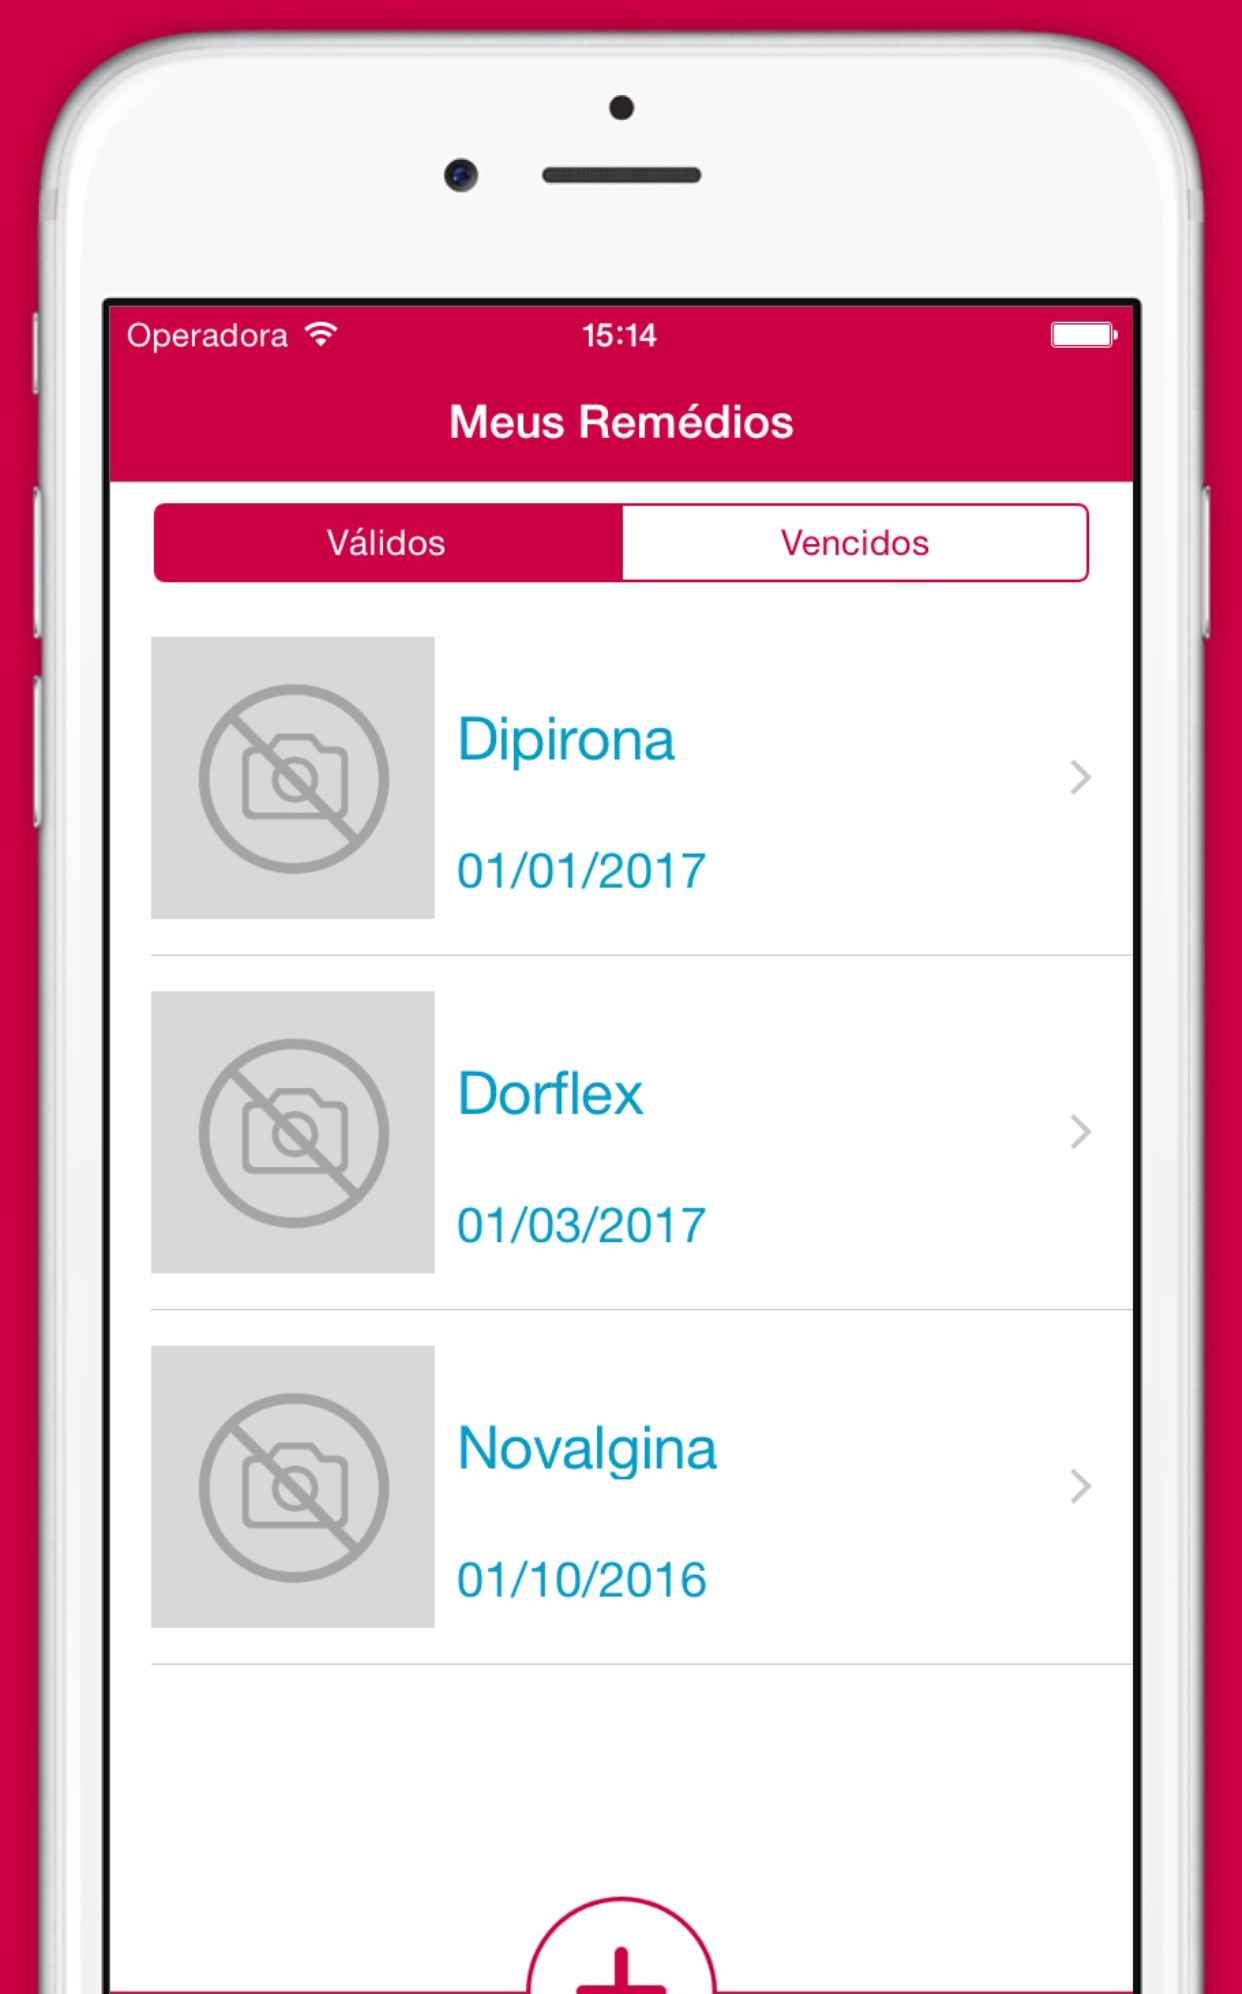
\includegraphics[width=0.5\textwidth]{minifarma}
    \caption[Tela inicial do aplicativo Mini Farma]{ Tela inicial do aplicativo Mini Farma.}
	\label{fig:minifarma}
\end{figure}

O aplicativo utiliza recursos nativos do sistema, os quais são descritos a seguir. 
\begin{itemize}
	\item \textbf{Localização geográfica}: Define a posição geográfica do dispositivo que o usuário está utilizando para salvar a 
    localização da farmácia onde ele comprou um medicamento para, caso seja necessário, explicar para alguém onde a 
    farmácia fica. Também é possível com base nessa localização da farmácia e do usuário, traçar uma rota para levá-lo diretamente à 
    farmácia em questão;
	\item \textbf{Notificações locais}: Diferente das notificações \textit{Push}, as notificações locais são criadas e agendadas na central 
    de notificações do dispositivo e o sistema se encarrega de entregá-las corretamente de acordo com parâmetros definidos pelo aplicativo. 
    No caso do Mini Farma, as notificações são usadas para lembrar o usuário, na data e hora corretas, de que o mesmo deve tomar seus medicamentos;
	\item \textbf{Ligação}: As notificações podem conter ações que executam um determinado bloco de código dentro do aplicativo. No Mini Farma, 
    uma das notificações possíveis é a de aviso de pouca quantidade ou remédio esgotado, no caso do medicamento ter acabado. 
    Quando essa notificação é enviada, pode ser feita uma ligação diretamente pela ação da notificação para o número da 
    farmácia cadastrado no aplicativo. Dessa forma, o usuário pode solicitar uma nova quantidade de medicamento diretamente com a farmácia. 
	\item \textbf{Câmera}: Para facilitar a identificação dos medicamentos, é possível tirar uma foto com a câmera do dispositivo para 
    cada remédio cadastrado. Além de uma foto para o medicamento em si, é possível tirar uma foto da receita dele, caso haja;
    \item \textbf{Rolo de câmera}: Se o usuário já tiver uma foto que o ajude a identificar o seu medicamento ou da receita do mesmo salva 
    no rolo de câmera, é possível escolher a foto sem precisar tirar uma nova;
\end{itemize}

Com exceção da Ligação, todos os outros recursos nativos do sistema precisam necessariamente serem autorizados pelo
usuário para funcionar. Caso o usuário não autorize, o aplicativo fica com funcionalidades reduzidas.

Como banco de dados foi usado o SQLite, por meio do \textit{framework} externo e \textit{open-source FMDB}\footnote{\url{https://github.com/ccgus/fmdb}}, 
disponível no Github;

A arquitetura do sistema foi criada com base no padrão de projeto \textit{MVC}, possuindo uma camada \textit{DAO (Data Access Object)} para comunicação 
com o banco de dados. No entanto, o \textit{MVC} tradicional difere em alguns aspectos do \textit{MVC} usado no iOS. 

No iOS, o \textit{MVC} trás uma controladora ligada à classe de \textit{view}, que é chamado de \textit{ViewController}, responsável por 
criar a ponte entre a interação do usuário pela \textit{view} com as classes modelos. Dessa forma, as \textit{ViewControllers} têm a 
responsabilidade de repassar as entradas do usuário para a \textit{model} e controlar a \textit{view} para apresentar os resultados que a modelo retornar.

Diferente do \textit{MVC} tradicional, no qual a controladora apenas repassa as informações que estão entrando na fronteira da aplicação, 
as \textit{ViewControllers} têm, além dessa responsabilidade, também a responsabilidade de instanciar e gerenciar a \textit{view} no tocante
à organização dos elementos e apresentação das informações.

Outra observação sobre as diferenças entre os dois \textit{MVCs}, é que no \textit{MVC} tradicional pode haver uma controladora apenas 
para todas as modelos ou uma controladora por modelo, mas nenhuma ligada diretamente a uma \textit{view}, no entanto, no iOS há uma 
\textit{ViewController} por \textit{view}, podendo haver ainda uma controladora relacionada com cada modelo conforme o padrão tradicional do \textit{MVC}.

\begin{figure}[h]
  \centering
    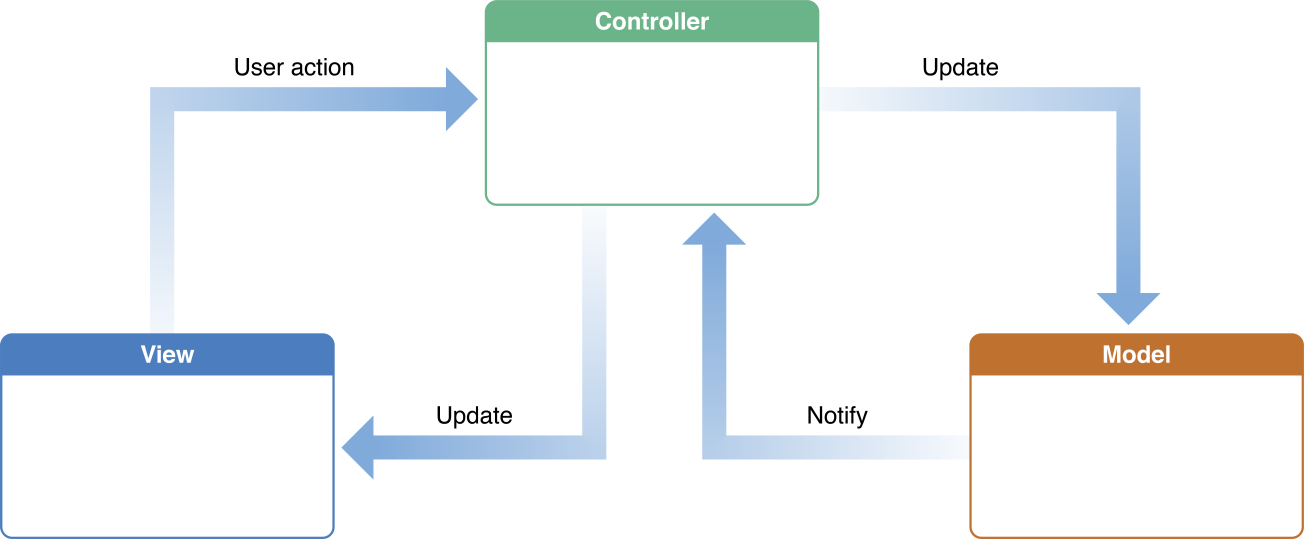
\includegraphics[width=1.0\textwidth]{mvc}
    \caption[Padrão \textit{Model-View-Controller}]{ Padrão \textit{Model-View-Controller}. Fonte: Apple Documentation.}
	\label{fig:mvc}
\end{figure}

\subsection{Ambiente de desenvolvimento} \label{subsec:ambientedesenvolvimento}
Nesta seção é apresentado todo o ambiente de desenvolvimento do \textit{app} Mini Farma quando foi feito originalmente para a plataforma iOS. 
O projeto foi executado contando com uma equipe de dois integrantes com conhecimentos intermediários na plataforma iOS. 
Os detalhes técnicos são listados a seguir.
\begin{itemize}
    \item \textbf{Máquinas}: Dois MacBook Pro Retina 13", processador \textit{Intel Core i5}, 8 GB de \textit{RAM};
    \item \textbf{Sistema Operacional das máquinas}: \textit{Mac OS X Yosemite} v10.10.5;
    \item \textbf{Sistema Operacional alvo do aplicativo}: iOS 8;
    \item \textbf{\textit{IDE}}: \textit{Xcode} v6.4;
    \item \textbf{Linguagem de Programação}: \textit{Swift} v1.3;
    \item \textbf{Banco de dados}: SQLite v3.8.10.2;
    \item \textbf{Ambiente de suporte}: \textit{Plugin SQLite Manager} para \textit{Mozilla Firefox}, para criação do banco de dados;
\end{itemize}

\section{Desenvolvimento multiplataforma do projeto} \label{sec:desenvolvimentomulti}

A partir do aplicativo feito em iOS, foi construída uma versão utilizando o Ionic para as plataformas Android e iOS, 
disponível em um repositório aberto no Github\footnote{\url{https://github.com/crossdev-tcc/ionic-apps}}. O desenvolvimento foi dividido nas seguintes funcionalidades:
\begin{itemize}
	\item \textbf{Listagem de Remédios e Alertas};
	\item \textbf{Cadastro de Remédios}: sendo necessário o acesso a câmera fotográfica e galeria de fotos do dispositivo;
	\item \textbf{Cadastro de Farmácias}: sendo necessário o acesso à localização do dispositivo e ligação de voz;
	\item \textbf{Cadastro de Alertas}: sendo necessário o acesso à central de notificações locais do dispositivo;
\end{itemize}
%\textit{* Todas as funcionalidades exigem acesso ao banco de dados local SQLite criado para o aplicativo}
Para a criação dessa versão do \textit{app}, a equipe foi alterada, mas permaneceu com dois integrantes, que são os autores deste trabalho.
No entanto, os integrantes não possuíam qualquer conhecimento prévio nos \textit{frameworks} Ionic, AngularJS e Cordova
e apenas possuíam um conhecimento básico em \textit{HTML}, \textit{CSS} e \textit{JavaScript}. Os detalhes técnicos são listados a seguir.
   
\begin{itemize}
    \item \textbf{Máquinas}: Dois MacBook Pro Retina 13", processador \textit{Intel Core i5}, 8 GB de \textit{RAM};
    \item \textbf{Sistema Operacional das máquinas}: \textit{Mac OS X El Capitan} v10.11.5;
    \item \textbf{Sistema Operacional alvo do aplicativo}: iOS 9.3 e Android 6.0.0;
    \item \textbf{\textit{IDE}}: \textit{WebStorm} v2016.1.1;
    \item \textbf{\textit{Frameworks}}:
    \begin{itemize}
        \item \textbf{Ionic}: \textit{Copenhagen} v1.2.4\footnote{Durante a execução deste trabalho, já haviam sido disponibilizadas as versões 2 do Ionic e do AngularJS, no entanto,
        	os autores optaram por não utilizá-las por ainda se tratarem de versões \textit{beta} e portanto instáveis, o que poderia 
        	impactar negativamente no desenvolvimento do projeto.\label{note1}};
        \item \textbf{AngularJS}: \textit{foam-acceleration} v1.4.3\footref{note1};
        
        \item \textbf{Cordova}: v6.0.0;
    \end{itemize}
    \item \textbf{Linguagem de Programação}: \textit{JavaScript} v1.7. 
    \begin{itemize}
        \item \textit{HTML} 5 e \textit{CSS} 3 foram usados paralelamente para a criação da interface gráfica do aplicativo;
    \end{itemize}
    \item \textbf{Banco de dados}: SQLite v3.8.10.2;
    \item \textbf{Ambiente de suporte}: Google Chrome, para \textit{debug} do aplicativo;
    \item \textbf{Simuladores}: 
    \begin{itemize}
        \item \textbf{iOS}: iPhone 6S Plus
        \item \textbf{Android}: Nexus 7
    \end{itemize}
\end{itemize}

\subsection{Relato de desenvolvimento} \label{subsec:experienciasdev}

É apresentado, a seguir, o relato das experiências obtidas durante o desenvolvimento com Ionic, dividido nas funcionalidades 
já descritas na Subseção~\ref{subsection:planejamentodesenvolvimento} deste trabalho, bem como feita a comparação entre o desenvolvimento nativo para iOS e 
o multiplataforma Ionic. Há, ainda, um tópico de observações gerais pertinentes à implementação do \textit{app} como um todo. 


 \begin{itemize}
 	
 	\item \textbf{Listagem de Remédios e Alertas};
		\begin{itemize}
			\item Para a tela inicial do \textit{app}, a lista de remédios e alertas, foi preciso realizar uma pequena alteração em relação ao original, para considerar, agora, 
			dois sistemas operacionais diferentes (iOS e Android). Foi preciso criar duas 
			\textit{views} para a mesma tela, pois o componente de abas (conhecido como \textit{tabs}), é diferente no iOS e no Android. Com isso, quando foi feito pensando-se no iOS do Ionic, ele não correspondia 
			muito bem ao padrão de interface do Android, por isso foi preciso criar duas telas separadas e fazer uma verificação se o dispositivo é iOS ou Android. Após feita a verificação de dispositivo, o próprio
			Ionic se encarrega de definir a aparência do componente para o padrão do sistema no qual o aplicativo está sendo executado.

			\item Para a criação da lista de remédios e alertas que o usuário possui cadastrados, o componente usado no iOS é chamado de \textit{UITableView}. No Ionic, o componente similar é o conjunto das diretivas 
			\textit{ion-list} e \textit{ion-item} do Ionic com a diretiva \textit{ng-repeat} do AngularJS. 
			É muito simples de ser implementada, possuindo documentação ampla e exemplos de uso nos \textit{sites} oficiais dos \textit{frameworks}.

			\item Para a realização das filtragens dos remédios por data de validade, e dos alertas por ativos e inativos, bastou usar o componente \textit{filter} padrão do AngularJS. Dessa forma, foi possível 
			mostrar apenas as informações que deveriam ser mostradas. Novamente, possuindo muitos exemplos e ajuda na documentação do \textit{framework}.

			 \begin{figure}[H]
			 	\centering
			 	\begin{minipage}{.5\textwidth}
			 		\centering
			 		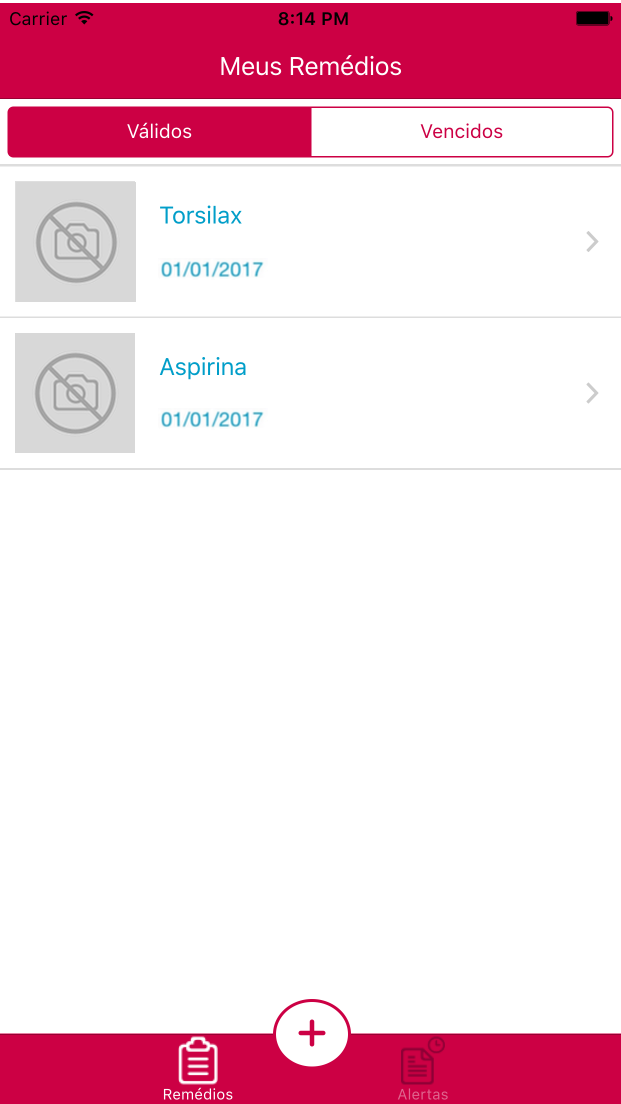
\includegraphics[width=.8\linewidth]{ionic_lista_ios}
			 	\end{minipage}%
			 	\begin{minipage}{.5\textwidth}
			 		\centering
			 		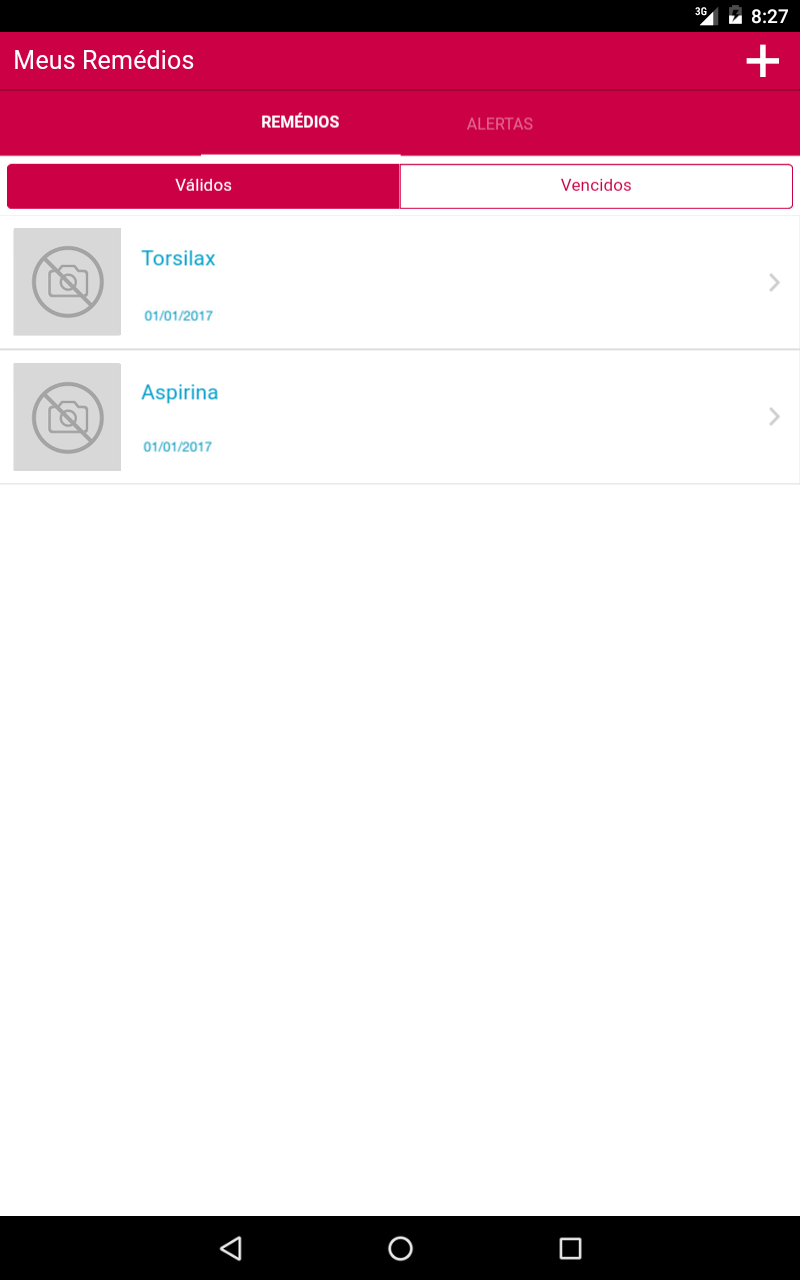
\includegraphics[width=0.9\linewidth]{ionic_lista_android}
			 	\end{minipage}
			 	\caption[Telas da lista de remédios (Ionic iOS \textit{versus} Ionic Android)]{ Telas da lista de remédios (Ionic iOS à esquerda \textit{versus} Ionic Android à direita).}
			 	\label{fig:ionic_lista}
			 \end{figure}

		\end{itemize}

 	\item \textbf{Cadastro de Remédios};
 	
 		 \begin{itemize}
			\item No cadastro de remédios há o uso da câmera do dispositivo para tirar uma foto do medicamento e para registrar a prescrição médica. Opcionalmente, pode-se selecionar as fotos a partir da biblioteca de imagens do dispositivo. Com o uso do \textit{plugin} Cordova de acesso à câmera, essa foi uma tarefa tranquila e que funcionou corretamente em ambas as plataformas, Android e iOS. 
			\item Para que o usuário opte entre  tirar uma nova foto e escolher da galeria do dispositivo, foi utilizado um componente conhecido no iOS como \textit{UIActionSheet}. Com o uso de um único código, o Ionic possibilitou a geração de um componente exatamente igual ao nativo do iOS e de um correspondente no Android. 
			Na Figura~\ref{fig:ionic_action_camera} é possível observar as diferenças de interface, as quais foram adequadas pelo Ionic para cada plataforma.
			
			 \begin{figure}
			 	\centering
			 	\begin{minipage}{.5\textwidth}
			 		\centering
			 		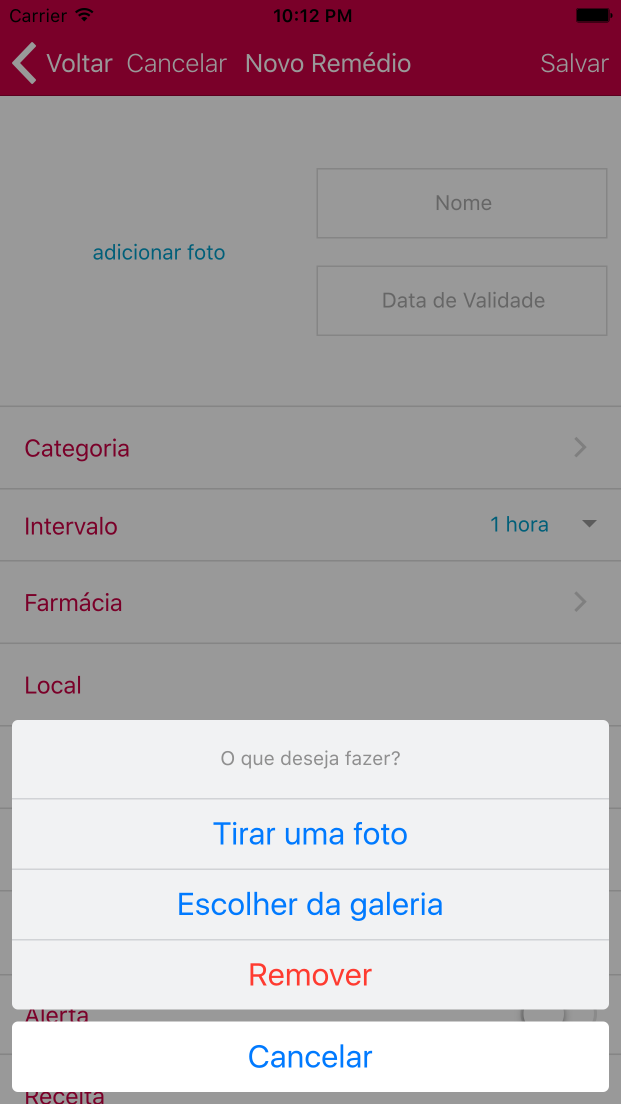
\includegraphics[width=.8\linewidth]{ionic_action_camera_ios}
			 	\end{minipage}%
			 	\begin{minipage}{.5\textwidth}
			 		\centering
			 		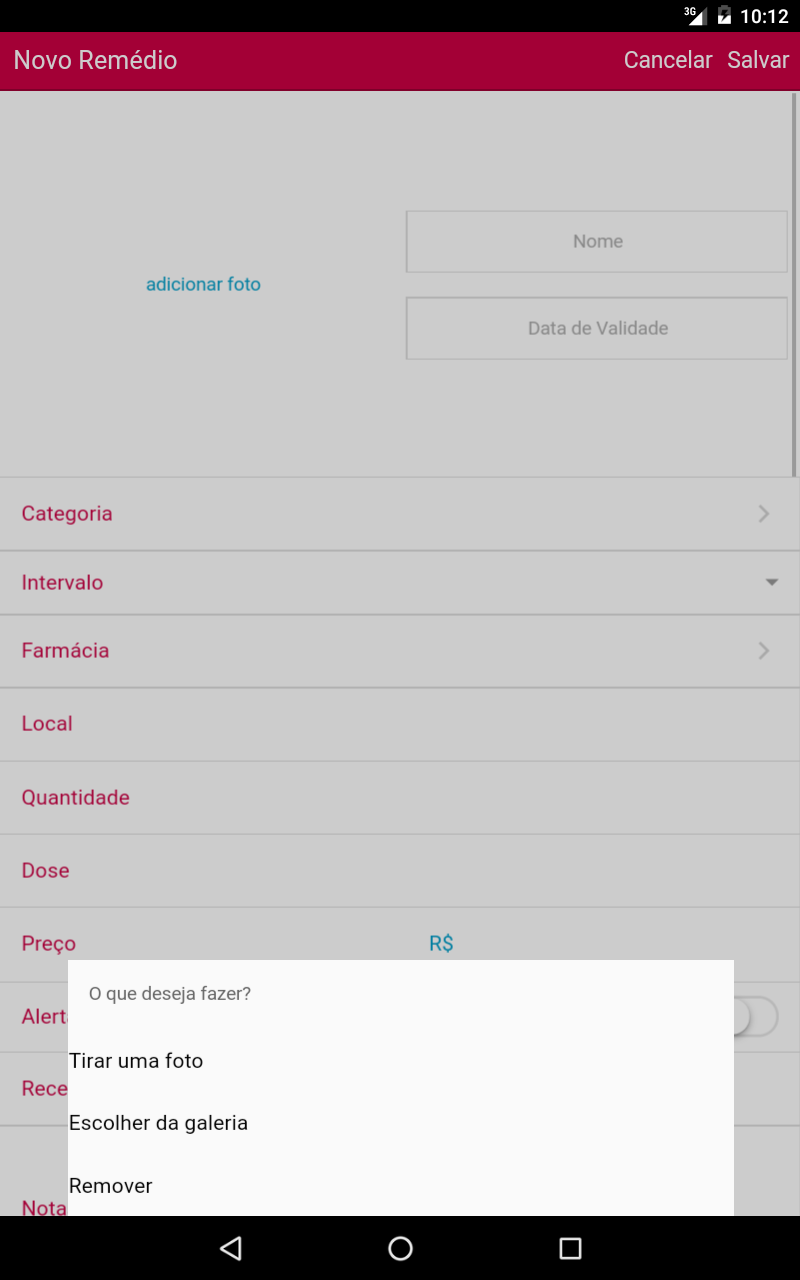
\includegraphics[width=0.9\linewidth]{ionic_action_camera_android}
			 	\end{minipage}
			 	\caption[Telas de cadastro de foto de remédio (Ionic iOS \textit{versus} Ionic Android)]{ Telas de cadastro de foto de remédio (Ionic iOS à esquerda \textit{versus} Ionic Android à direita).}
			 	\label{fig:ionic_action_camera}
			 \end{figure}

			\item Outro componente utilizado e propriamente adaptado pelo Ionic para as plataformas foi o denominado no iOS como \textit{UIPickerView}.
			Ele foi utilizado para a escolha de intervalo de uso do medicamento e é apresentado na Figura~\ref{fig:ionic_picker}.
			 
			 \begin{figure}
			 	\centering
			 	\begin{minipage}{.5\textwidth}
			 		\centering
			 		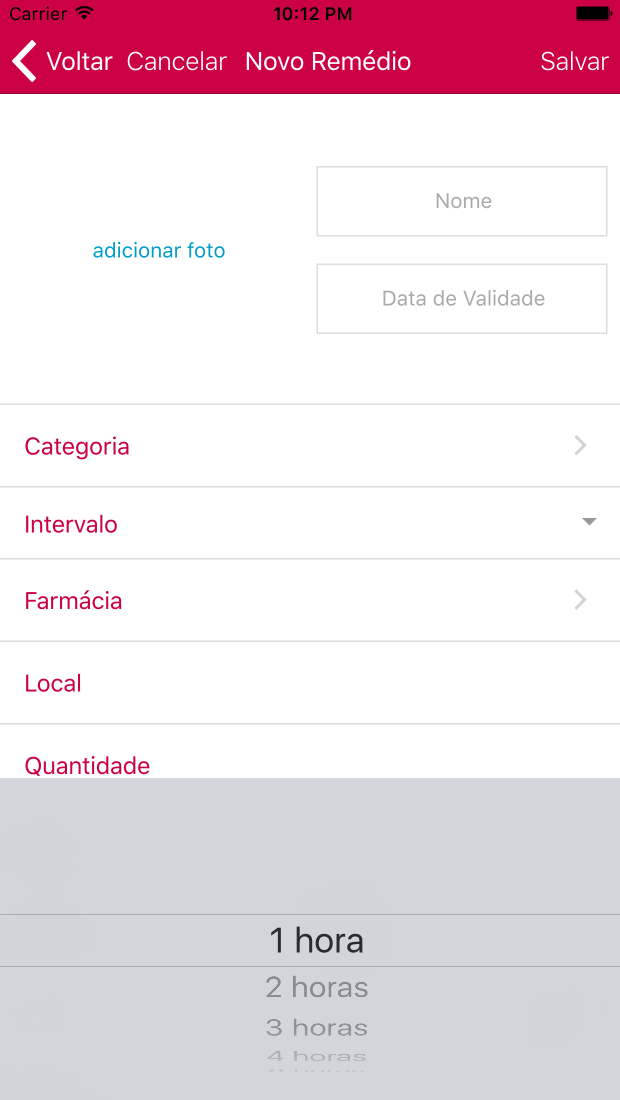
\includegraphics[width=.8\linewidth]{ionic_picker_ios}
			 	\end{minipage}%
			 	\begin{minipage}{.5\textwidth}
			 		\centering
			 		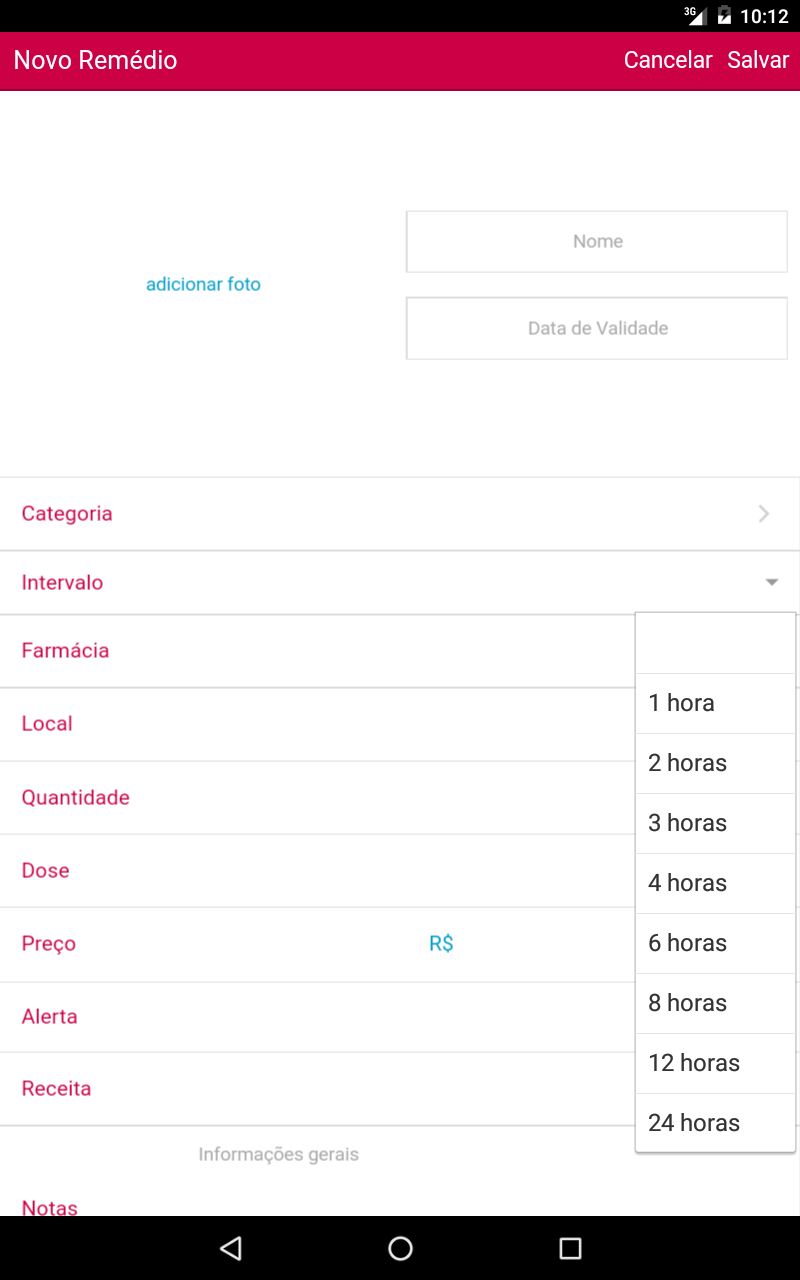
\includegraphics[width=0.9\linewidth]{ionic_picker_android}
			 	\end{minipage}
			 	\caption[Telas de cadastro de intervalo de remédio (Ionic iOS \textit{versus} Ionic Android)]{ Telas de cadastro de intervalo de 
				 remédio (Ionic iOS à esquerda \textit{versus} Ionic Android à direita).}
			 	\label{fig:ionic_picker}
			 \end{figure}
			 
		 	\item No formulário de cadastro há a opção de selecionar uma categoria para o medicamento, para isso, o usuário é direcionado a uma página que contém a lista de categorias disponíveis, seleciona alguma delas ou adiciona uma nova e é redirecionado à página de cadastro, com o campo de categoria preenchido com a escolha feita. Para isso é necessário o envio de dados de uma tela para a antecessora. No aplicativo nativo, essa funcionalidade foi implementada com o uso dos chamados \textit{Protocols and Delegates}. Já no aplicativo multiplataforma, não foi encontrada uma correspondência aos protocolos do iOS, foi, então, utilizada uma \textit{factory} para armazenar temporariamente o valor da categoria. Observou-se que o nível de dificuldade de ambas as abordagens é semelhante, não apresentando grande dificuldade de implementação.
			 
			\item Para a criação de uma nova categoria de remédios, foi utilizada uma interação por meio de uma caixa de diálogo, também conhecida como alerta. Para isso, utilizou-se os chamados \textit{popups} do Ionic.  Apesar de facilmente implementados e personalizáveis, esses componentes não se assemelham às caixas de diálogo nativas do iOS, \textit{UIAlertView} e do Android, \textit{AlertDialog}. O alerta criado é apresentado na Figura~\ref{fig:ionic_alert}. Posteriormente,  foi verificado que há no Cordova uma \textit{API} para caixas de diálogo que, diferente da disponibilizada pelo Ionic, gera uma interface adequada aos padrões de ambas as plataformas. Um exemplo de alerta  gerado pelo Cordova e idêntico à uma das plataformas, neste caso o iOS, é apresentado na Figura~\ref{fig:ios_prompt}.
			 	
			 	\begin{figure}[H]
			 		\centering
			 		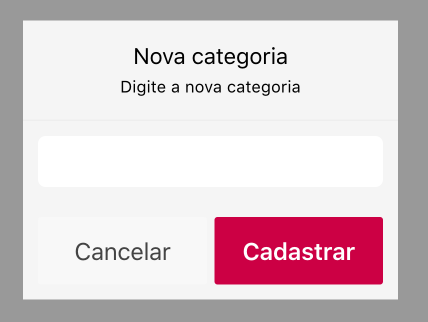
\includegraphics[width=0.5\textwidth]{ionic_alert}
			 		\caption[Tela de alerta - Ionic]{Tela de alerta - Ionic.}
			 		\label{fig:ionic_alert}
			 	\end{figure}
			 	
			 	\begin{figure}[H]
			 		\centering
			 		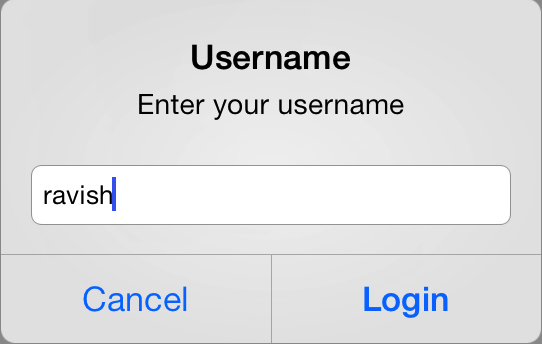
\includegraphics[width=0.5\textwidth]{ios_prompt}
			 		\caption[Alerta Cordova - iOS nativo]{Alerta Cordova - iOS nativo. Fonte: \cite{framework_ngcordova_2016}.}
			 		\label{fig:ios_prompt}
			 	\end{figure}
			 	
			 	%\item  Para o registro de local de armazenamento, quantidade e dose do remédio foram feitas campos colapsáveis
			 	%Mais facil, nao foi necessario alterar tamanho da celula, pois ao esconder o elemento a view se adaptada ao tamanho sem ele.
			 	
			 	\item Para a seleção do local de armazenamento do remédio foi utilizado um componente inexistente no iOS, que é uma caixa de seleção. O resultado não agradou muito por ter ficado com aspecto de componente \textit{web} e por não ter lembrado nenhum dos componentes nativos do iOS. Já para a plataforma Android o resultado foi satisfatório. O componente é apresentado na Figura~\ref{fig:ionic_local}.
			 	
			 		 \begin{figure}[H]
			 		 	\centering
			 		 	\begin{minipage}{.5\textwidth}
			 		 		\centering
			 		 		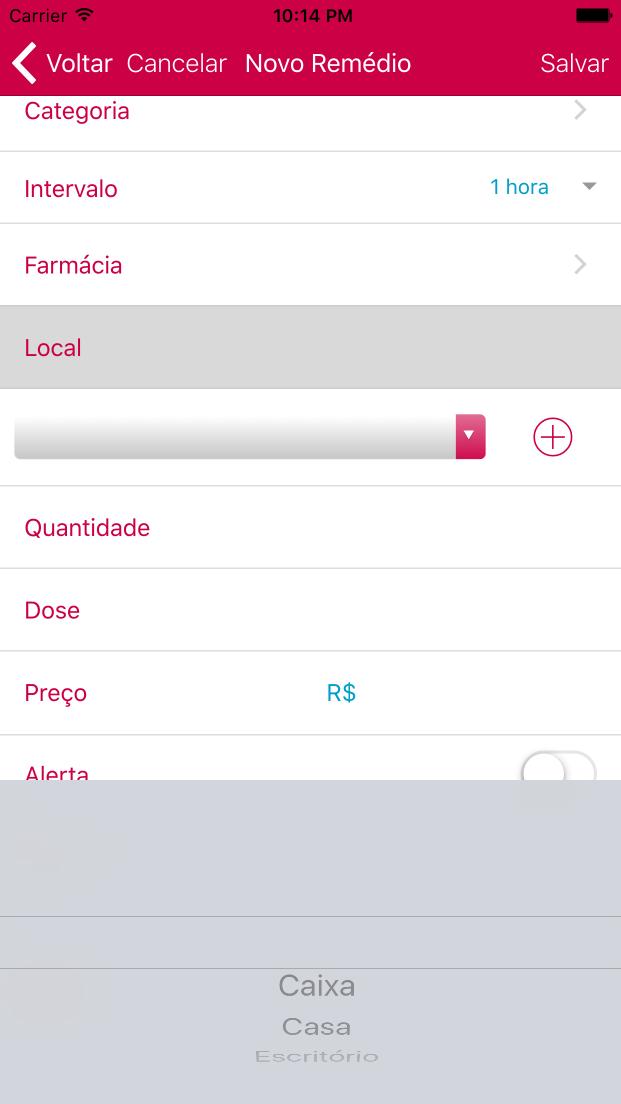
\includegraphics[width=0.8\linewidth]{ionic_local_ios}
			 		 	\end{minipage}\hfill
			 		 	\begin{minipage}{.5\textwidth}
			 		 		\centering
			 		 		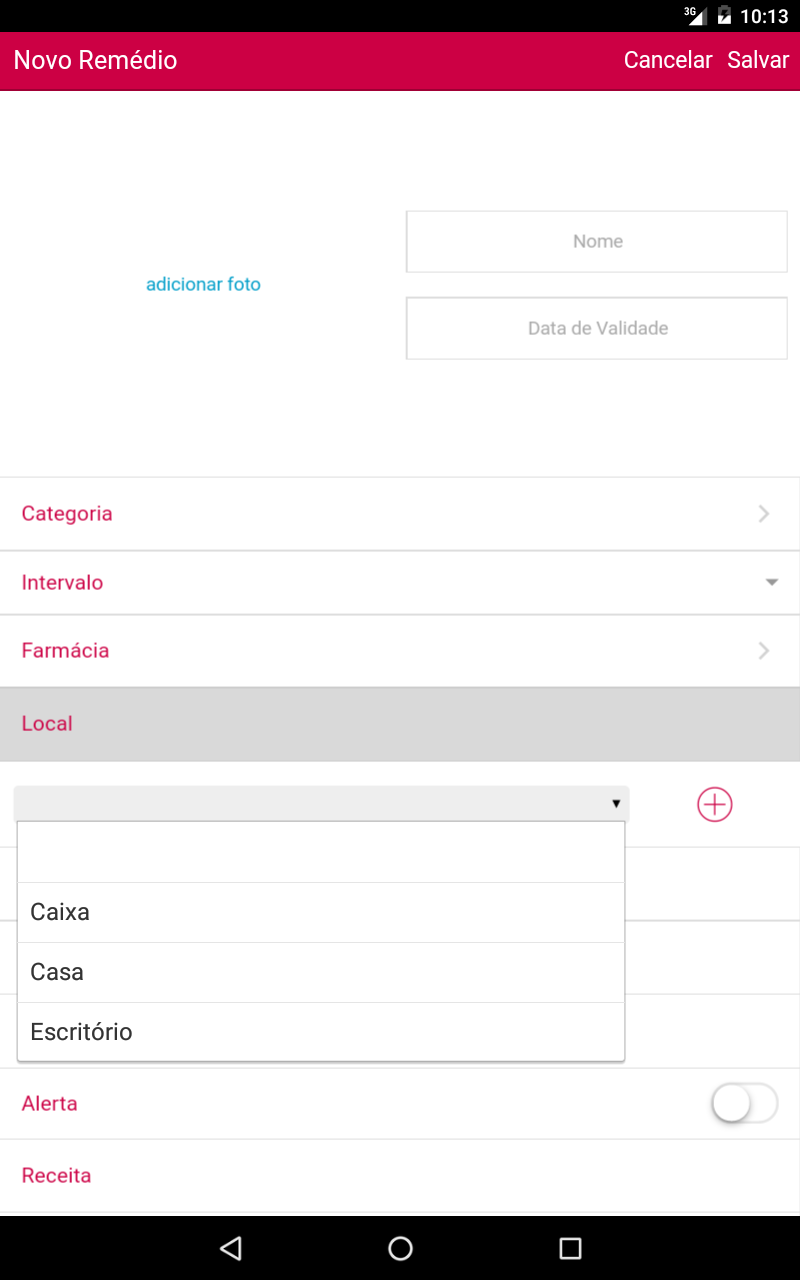
\includegraphics[width=0.9\linewidth]{ionic_local_android}
			 		 	\end{minipage}
			 		 	\caption[Tela de cadastro de local do remédio  (Ionic iOS \textit{versus} Ionic Android)]{ Tela de cadastro de local do remédio  (Ionic iOS à esquerda \textit{versus} Ionic Android à direita).}
			 		 	\label{fig:ionic_local}
			 		 \end{figure}
			 	
		 		\item Em relação ao banco de dados, utilizou-se a \textit{API} Cordova SQLite. Como o banco de dados 
		 		construído nativamente também foi feito utilizando o SQLite, foi possível aproveitar os \textit{scripts} 
		 		de definição e manipulação de dados. Não houveram complicações no uso da \textit{API} e facilmente 
		 		foram encontrados exemplos de uso na internet que auxiliaram na estruturação da camada de comunicação 
		 		do aplicativo com o banco de dados.
		 		
		 		\item De forma geral, o resultado da tela de cadastro de remédios foi satisfatório e a interface construída ficou semelhante à tela do aplicativo nativo, apresentado na Figura~\ref{fig:ios_cadastro_remedio}. A tela construída com Ionic é apresentada nas Figuras ~\ref{fig:ionic_action_camera} e ~\ref{fig:ionic_local}.
		 		
		 			 	\begin{figure}[H]
		 			 		\centering
		 			 		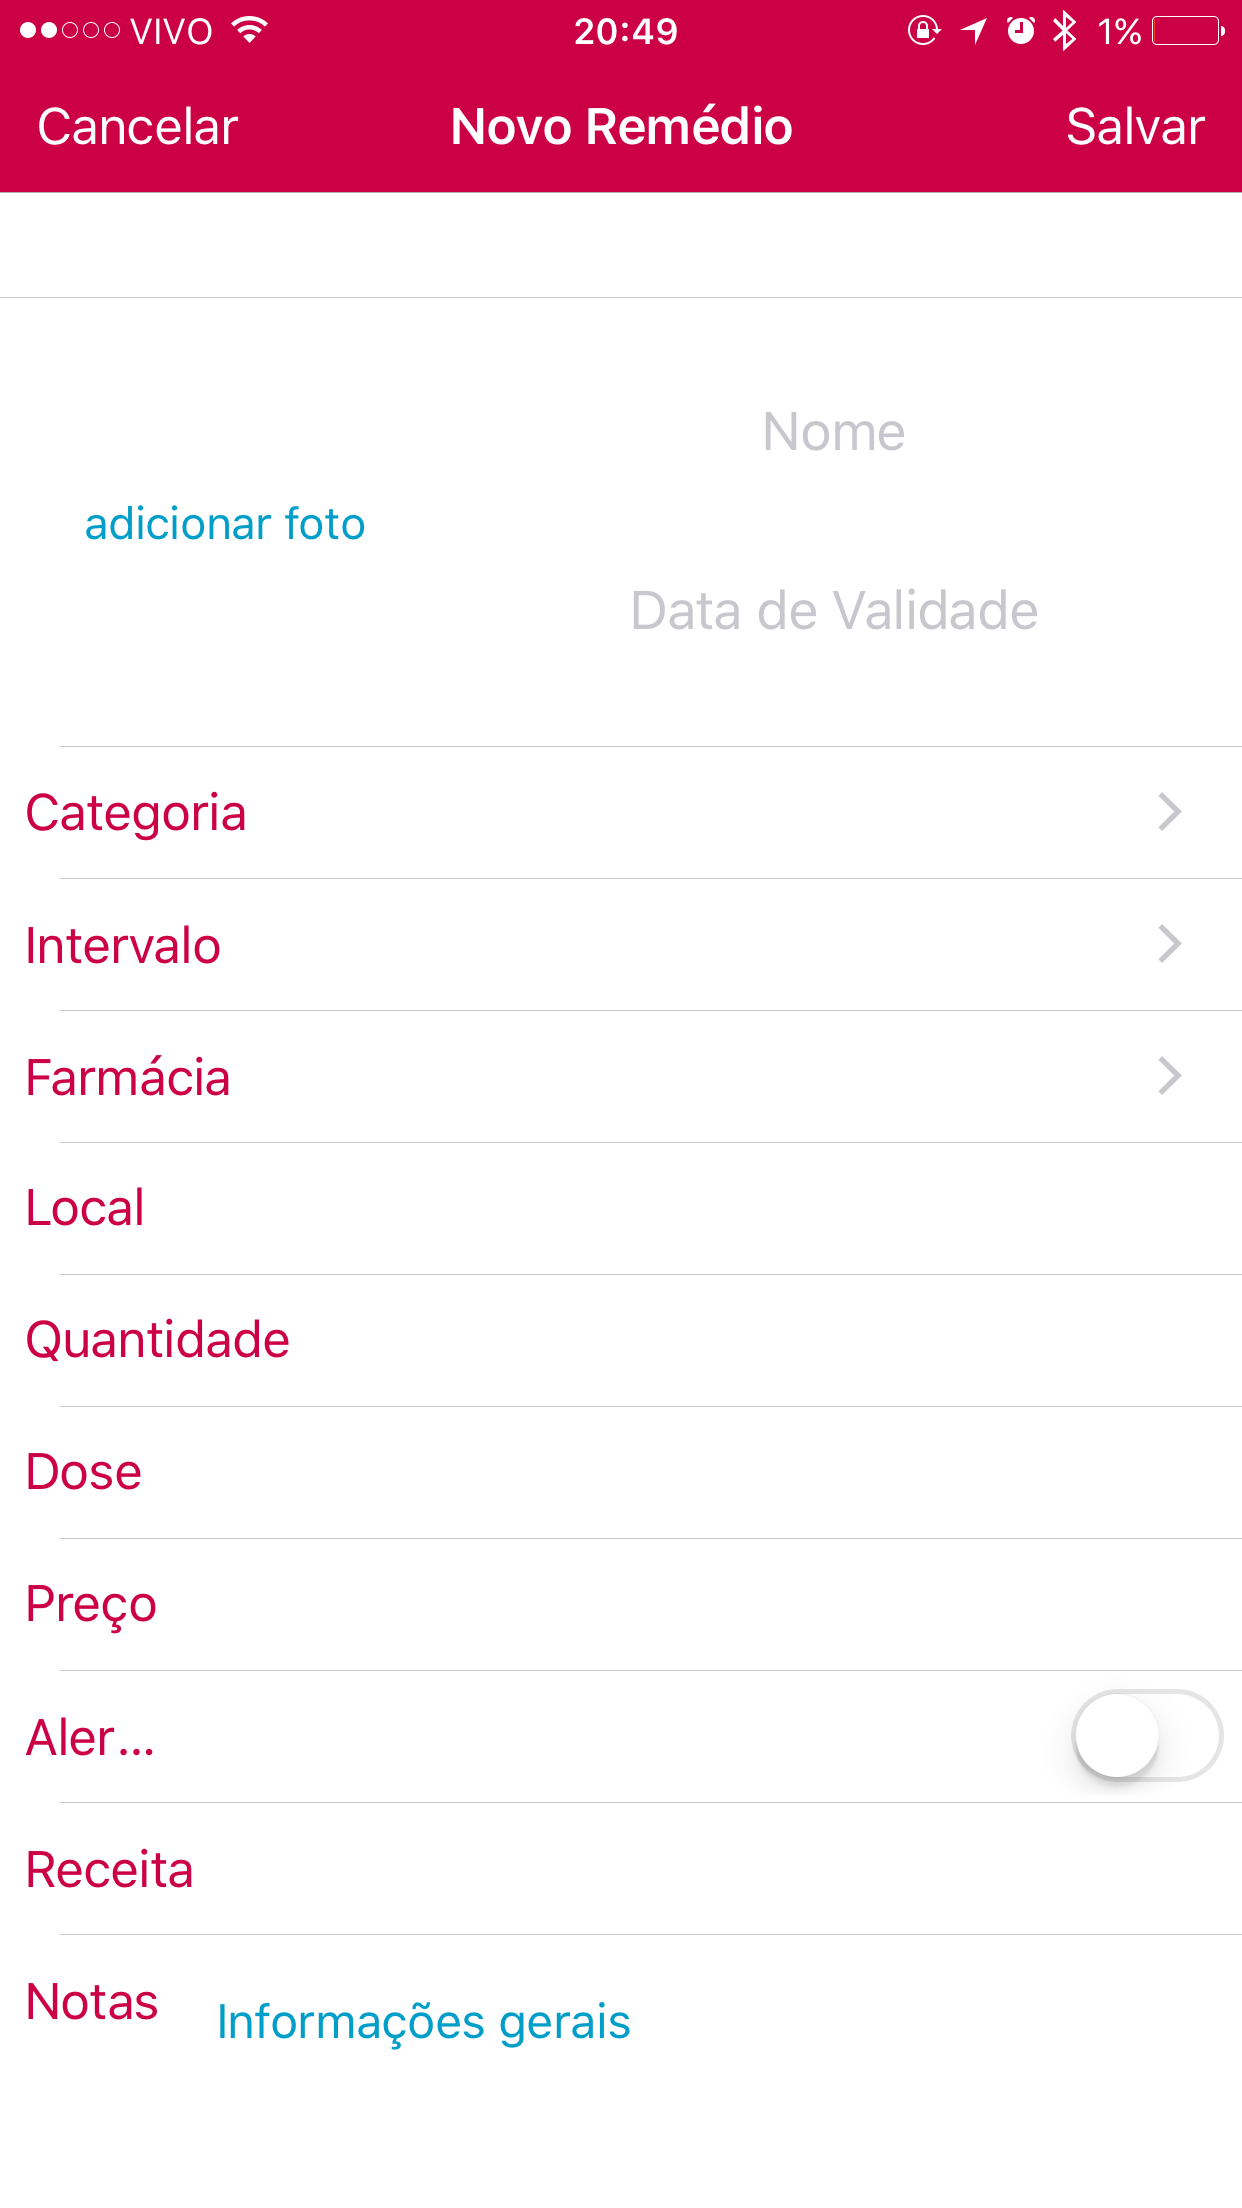
\includegraphics[width=0.4\textwidth]{ios_cadastro_remedio}
		 			 		\caption[Tela de cadastro de remédio - iOS]{Tela de cadastro de remédio - iOS nativo.}
		 			 		\label{fig:ios_cadastro_remedio}
		 			 	\end{figure}
			 
		 \end{itemize}
     \item \textbf{Cadastro de Farmácias}; 	
	 \begin{itemize}
		\item Para cadastrar uma nova farmácia, o usuário deve marcar no mapa onde a farmácia se encontra. Para a utilização do mapa no Ionic, foi utilizada a \textit{API Maps} do Google, diferentemente da 
		\textit{API MapKit} do iOS. Não houveram grandes dificuldades na criação do mapa e renderização do mesmo na tela. A dificuldade de implementação é similar a do iOS nativo.
		Apenas realizando pesquisas e estudos na documentação da \textit{API} do Google, 
		já foi possível a elaboração do que precisava ser feito, no caso, mostrar o mapa e fornecer a opção de mover o pino para um local específico e capturar as coordenadas daquele ponto. No caso, foi 
		necessário utilizar a diretiva \textit{map} para renderização do mapa na tela e definir o \textit{callback} de reposicionamento do cursor e captura da localização. Na Figura~\ref{fig:add_farma} é possível 
		ver as diferenças entre o mapa do \textit{MapKit} do iOS e da \textit{API Maps} do Google.
	 \end{itemize}
	 \begin{figure}[H]
		\centering
		\begin{minipage}{.5\textwidth}
			\centering
			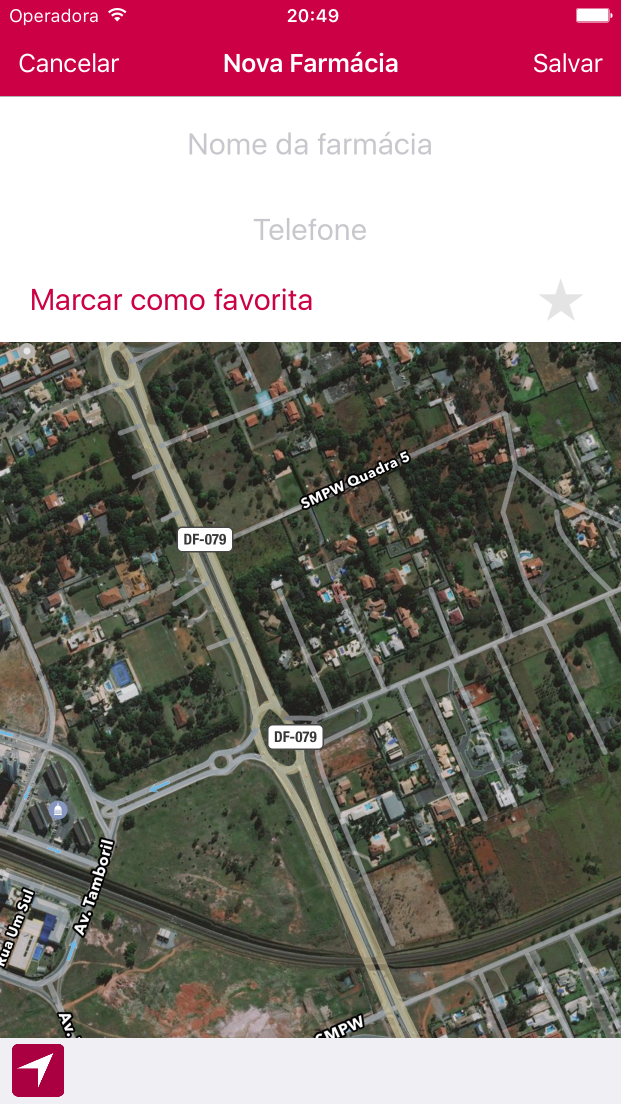
\includegraphics[width=0.9\linewidth]{ios_add_farma}
		\end{minipage}\hfill
		\begin{minipage}{.5\textwidth}
			\centering
			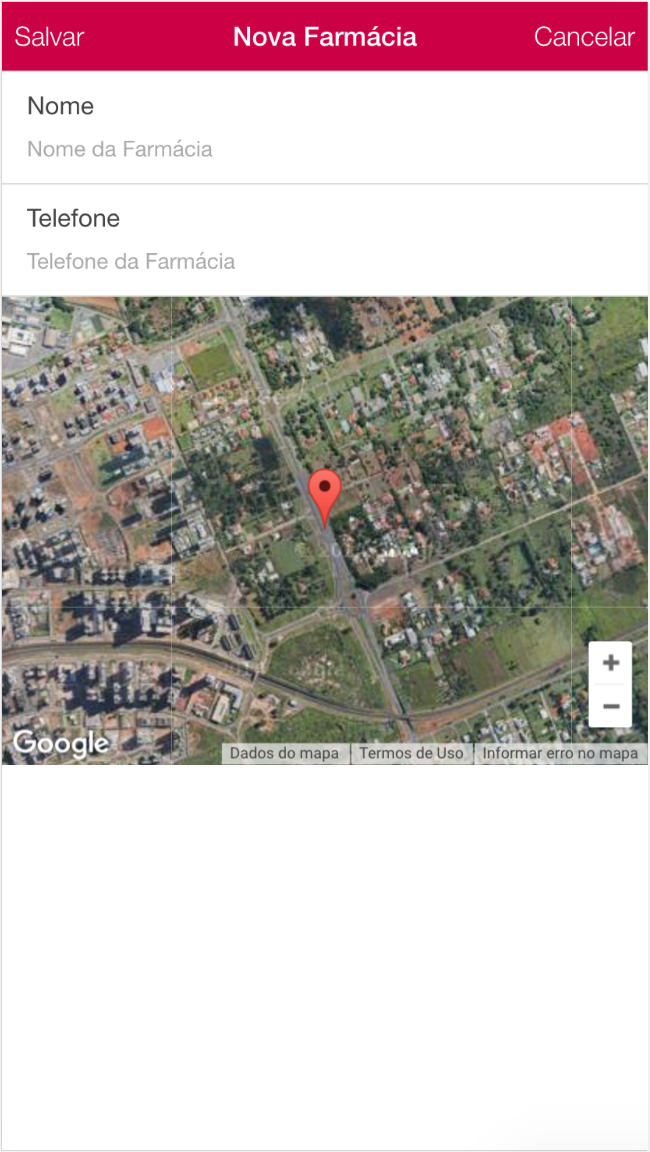
\includegraphics[width=0.9\linewidth]{ionic_add_farma}
		\end{minipage}
	\caption[Tela de adicionar farmácia (iOS \textit{versus} Ionic)]{ Tela de adicionar farmácia (iOS nativo à esquerda \textit{versus} Ionic iOS à direita).}
	\label{fig:add_farma}
	\end{figure}
 	
 	\item \textbf{Cadastro de Alertas};
 	
	\begin{itemize}
		\item Para o cadastro de um novo alerta, é preciso selecionar data e hora que o usuário será alertado. Para isso, o Ionic 1 não possui o componente adequado. Com isso, foi necessário procurar 
		e utilizar um \textit{framework} terceiro. Os \textit{frameworks} escolhidos foram o \textit{ionic-datepicker}\footnote{\url{https://github.com/rajeshwarpatlolla/ionic-datepicker}} e 
		\textit{ionic-timepicker}\footnote{\url{https://github.com/rajeshwarpatlolla/ionic-timepicker}}, respectivamente para seleção de data e hora. Ambos foram desenvolvidos pelo mesmo usuário no Github 
		e instalados no projeto do aplicativo via \textit{CLI}. Nas próprias documentações dos \textit{frameworks} existem exemplos de uso suficientes para guiar a implementação das funcionalidades. 
		Vale ressaltar que o componente \textit{DatePicker} do iOS permite a seleção de data e hora ao mesmo tempo, enquanto nos \textit{frameworks} utilizados, a seleção de data e hora é separada em dois componentes distintos, 
		gerando uma pequena alteração na interface gráfica da tela de cadastro de alertas quando comparada com a do aplicativo original. As diferenças entre o original e Ionic podem ser vistas na 
		Figura~\ref{fig:dateTimePicker}. O mesmo \textit{framework} para seleção de data também foi utilizado na tela de cadastro de remédios para definir a data de validade do mesmo.

		\item Para a criação dos alertas é preciso cadastrar notificações locais na central de notificações do dispositivo. Realizar essa tarefa teve o mesmo nível de dificuldade da implementação no iOS nativo. 
		Apenas foi instalado um \textit{plugin} do Cordova para gerenciar a central de notificações e agendar notificações com as datas e horas corretas para serem entregues. 
	\end{itemize}

	\begin{figure}[H]
		\centering
		\begin{minipage}{.33\textwidth}
			\centering
			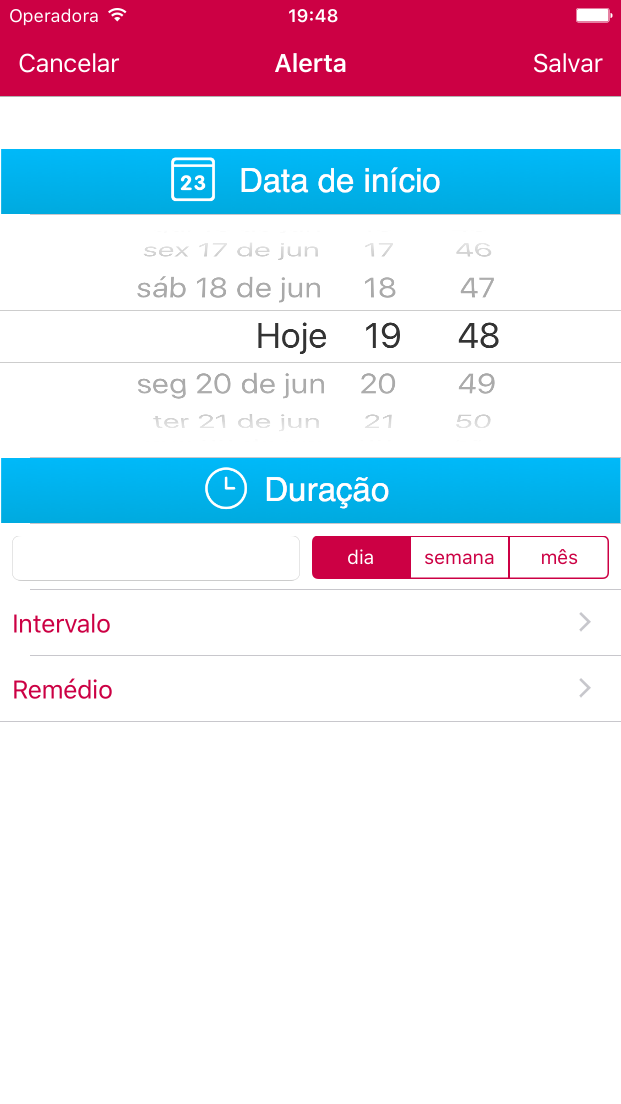
\includegraphics[width=0.95\linewidth]{ios_datetimepicker}
		\end{minipage}%
		\begin{minipage}{.33\textwidth}
			\centering
			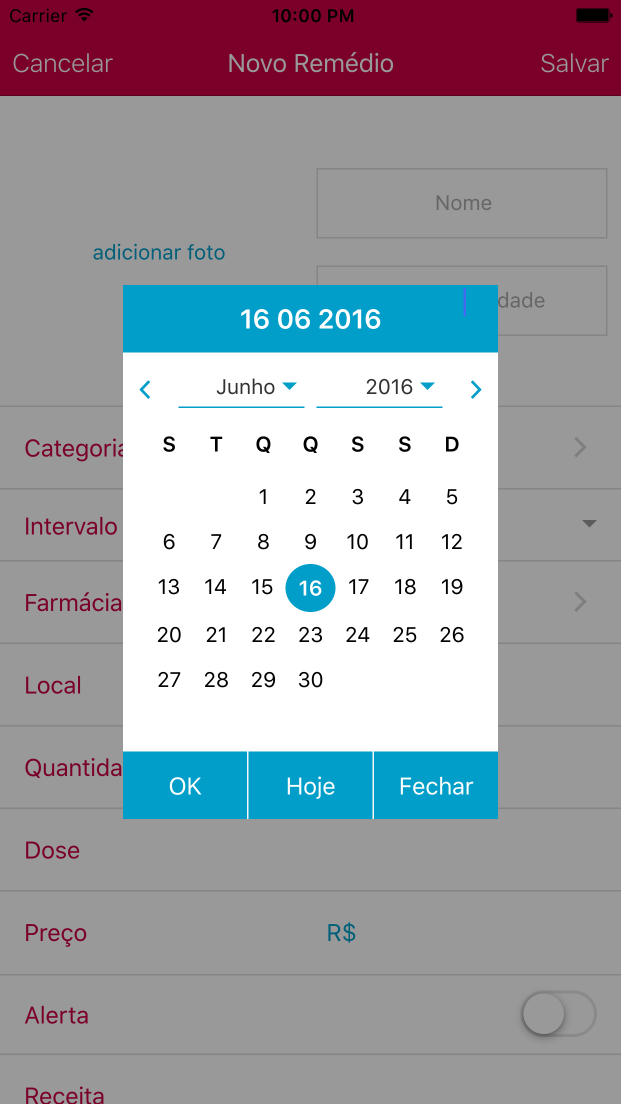
\includegraphics[width=0.95\linewidth]{ionic_datepicker}
		\end{minipage}
	\caption[Seleção de data e hora dos alertas (iOS \textit{versus} Ionic)]{ Seleção de data e hora dos alertas (iOS nativo à esquerda \textit{versus} Ionic iOS à direita).}
	\label{fig:dateTimePicker}
	\end{figure}
 	
 	\item \textbf{Observações gerais};
	\begin{itemize}
		\item Houve um problema no carregamento da lista inicial de remédios. Por ficar na primeira tela do aplicativo, acontecia de o acesso ao banco de dados para obtenção da lista ocorrer antes do total carregamento do Ionic, o que 
		acarretava em falha na execução do aplicativo. Esse problema não existiu na criação do \textit{app} original e para contorná-lo foram feitas pesquisas na comunidade para saber como resolver.
		Umas das soluções sugeridas era causar um \textit{delay} proposital no aplicativo para que desse tempo do Ionic carregar completamente, mas foi descartada para não impactar negativamente na performance do
		\textit{app}. A solução utilizada foi fazer uma verificação a cada transação realizada no banco de dados para que só sejam efetuadas caso o Ionic esteja pronto para ser usado e apresentado.
		\item O Ionic apresenta uma útil funcionalidade que permite o \textit{debug} dos aplicativos pelo terminal, porém, a partir da versão 9 no iOS não é possível realizar essa ação, enquanto que no Android continua funcionando adequadamente.
		Para corrigir o problema, usuários do Ionic recomendam a modificação de uma configuração no arquivo \textit{.plist} do projeto iOS, para desabilitar a opção \textit{App Transport Security} e permitir requisições que não  sejam \textit{HTTPS}. No entanto, ao modificar essa opção há o risco do aplicativo ser recusado no momento da sua publicação, portanto é necessário lembrar de reabilitá-la antes de submeter para a loja de aplicativos.
		Caso opte-se por não realizar essa alteração, para debugar é preciso um computador com \textit{Xcode} ou é possível também utilizar os navegadores como \textit{Google Chrome} ou \textit{Safari}
		no modo desenvolvedor para debugar utilizando o console \textit{JavaScript} dos navegadores.
		\item Alguns erros do \textit{JavaScript} não são acusados pelo terminal do Ionic, dificultando a tarefa de \textit{debug} da aplicação. 
		Com isso, em um momento de dificuldade em achar um problema que estava acontecendo, algumas pesquisas foram realizadas na comunidade \textit{on-line} e em um fórum 
		de discussão sobre Ionic foi dada uma dica sobre o uso de alertas do \textit{JavaScript} para mostrar erros para o desenvolvedor e com isso facilitar na tarefa de debugar o aplicativo.
		\item A diretiva \textit{ng-class} do AngularJS não funciona em conjunto com a diretiva \textit{ion-nav} do Ionic. No entanto, isso não foi achado nas documentações, nem do Ionic e nem do AngularJS. 
		Novamente, recorremos à comunidade e foi dito que esses componentes não funcionam corretamente juntos.
		\item Por mais que os autores não possuíssem conhecimentos avançados em \textit{HTML}, \textit{CSS} e \textit{JavaScript}, vale ressaltar que o conhecimento inicial nessas tecnologias ajudou muito 
		durante o desenvolvimento do \textit{app}.
		\item O Cordova e o Ionic possuem documentações bem completas, apresentando exemplos de uso de códigos. A comunidade é ativa e disponibiliza \textit{APIs} adicionais e exemplos de códigos em repositórios online.
	\end{itemize}
 \end{itemize} 

Apesar das desvantagens citadas na Tabela~\ref{tab:vantxdesva}, não houveram limitações quanto ao uso dos recursos necessários para o projeto 
ou problemas de performance que impactassem nos requisitos do aplicativo.
Foi possível construir apenas um código e gerar dois executáveis de plataformas diferentes, o que poderia acarretar em redução de custos e tempo de desenvolvimento.
Além disso o aplicativo desenvolvido apresentou aparência e usabilidade semelhantes ao nativo, adaptando-se a cada plataforma alvo seguindo seus padrões específicos de interface de usuário.

\subsection{Comparação de funcionalidades} \label{subsec:comparacaofuncionalidades}

Foram selecionadas algumas funcionalidades muito comuns em aplicativos para serem comparadas tecnicamente entre iOS, Android e Ionic, com o objetivo de melhorar o embasamento para a tomada de decisão entre o desenvolvimento 
nativo e multiplataforma. Importante ressaltar que para o aplicativo Ionic utilizar os recursos do celular, tanto \textit{hardware} quanto \textit{software}, é sempre necessária a utilização de 
\textit{plugins} do Cordova, ou seja, sempre que um novo recurso for desenvolvido para um dispositivo, há um tempo de espera para a criação do \textit{plugin} necessário para utilizar o novo recurso, 
e se o \textit{plugin} for descontinuado, eventualmente poderá quebrar a aplicação e prejudicar a experiência do usuário. A seguir são apresentados trechos de códigos, minerados de repositórios públicos e criados 
pelos autores, comentados para facilitar o entendimento das funcionalidades. 

\subsubsection{Login com Facebook} \label{subsubsec:loginfb}
Independente da plataforma, sempre deve haver um passo anterior ao desenvolvimento desta funcionalidade que é o registro do 
aplicativo a ser desenvolvido na plataforma para desenvolvedores do Facebook\footnote{\url{https://developers.facebook.com}}. O registro do aplicativo deve ser feito
para cada plataforma que se deseja atingir, por exemplo, iOS e Android, utilizando para isso, o nome do pacote do aplicativo em cada plataforma.
%Por exemplo, na criação do aplicativo iOS é definido um \textit{bundle ID}, já no Android é definido um nome do pacote. 

Com esta estapa concluída, pode-se iniciar o desenvolvimento desta funcionalidade utilizando para isso o \textit{SDK} do Facebook para iOS e Android.
No caso do Ionic, existem alguns \textit{plugins} que podem ser utilizados, como por exemplo o \textit{\$cordovaOauth}\footnote{\url{http://ngcordova.com/docs/plugins/oauth/}}, disponível dentro do próprio ngCordova, 
que permite a conexão com vários provedores de serviços, tais como Google, Github, Facebook e Linkedin, por exemplo. 

Além desse, existem outros meios de se conectar aos provedores, por exemplo, utilizando o 
Firebase\footnote{\url{https://www.firebase.com}} do Google. Desta forma, é possível acessar os dados públicos do usuário como nome, e-mail e foto de perfil para realizar um cadastro e \textit{login} no aplicativo.
Em todas as três plataformas citadas (iOS, Android e Ionic), a complexidade é similar, havendo apenas diferenças inerentes a cada linguagem e plataforma. 

Vale ressaltar, que o \textit{login} com redes sociais, nada mais é do que a obtenção dos dados do usuário de uma plataforma terceira por meio do protocolo \textit{OAuth}, 
ou seja, não são criadas sessões a partir das plataformas terceiras, apenas os dados do usuário na outra plataforma são acessados para que não haja a necessidade do usuário informá-los novamente. A partir dos dados 
obtidos, o aplicativo se encarrega de realizar o cadastro e \textit{login} do usuário de acordo com as regras de negócio do aplicativo. 
A seguir são apresentados dois trechos de código no iOS e no Ionic para \textit{login} com o Facebook. No iOS foi utilizado o \textit{SDK} nativo do Facebook, já no Ionic, foi utilizado o \textit{Firebase}. 

\begin{figure}[H]
	\centering
	\includegraphics[width=1\textwidth]{codes/ios/loginfb}
	\caption[Requisição de dados do Facebook no iOS]{Requisição de dados do Facebook no iOS}
	\label{fig:loginfb-ios}
\end{figure}

\begin{figure}[H]
	\centering
	\includegraphics[width=1\textwidth]{codes/ionic/loginfb}
	\caption[Requisição de dados do Facebook no Ionic]{Requisição de dados do Facebook no Ionic. Fonte: Baseado em Github\protect\footnotemark}
	\label{fig:loginfb-ios}
\end{figure}

\footnotetext{\url{https://github.com/fga-gpp-mds/2016.1-Partiu_frontend}}

Vale ressaltar que o \textit{plugin} do Cordova é genérico para vários provedores, ou seja, com o mesmo código é possível requisitar os dados em vários serviços distintos. Já nos \textit{SDKs} nativos, isso não ocorre.
Caso haja a necessidade de obtenção de dados de vários provedores, como por exemplo, no caso de \textit{login} com Facebook e Google, na abordagem nativa é preciso utilizar a \textit{SDK} do Facebook para iOS e Android
e a \textit{SDK} do Google para iOS e Android. O mesmo não ocorre no multiplataforma, pois com o mesmo \textit{plugin} é possível fazer a conexão com vários serviços apenas alterando uma \textit{string}, 
o que pode tornar o desenvolvimento mais simples que na abordagem nativa.

\subsubsection{Consumo de Web Services} \label{subsubsec:webservices}
Como o poder computacional dos dispositivos móveis, embora elevado, ainda não é comparável ao dos servidores, muitos aplicativos utilizam um modelo cliente/servidor, no qual
as operações mais custosas computacionamente são processadas no lado servidor e não no cliente. Além disso, a persistência dos dados da aplicação dificilmente é feita localmente nos dispositivos para evitar 
perdas de dados no caso de roubos, extravios ou danos ao aparelho, facilitar a migração para outros dispositivos e o uso em outras plataformas. Com isso, é necessário que os aplicativos estejam preparados para se 
comunicarem com \textit{Web Services}. Para realizar essa comunicação, cada plataforma oferece alguns meios nativos como classes e \textit{frameworks}, no entanto, existem \textit{frameworks} de terceiros que 
são muito utilizados e conhecidos na comunidade de desenvolvedores tanto para comunicar com os \textit{Web Services}, como para lidar com JSON e XML usados na comunicação entre aplicativo/servidor. 

Para realizar essa atividade no Ionic, o AngularJS dispõe do \textit{plugin ngResource} muito conhecido e utilizado para interação com \textit{web services}. Ele trás o objeto \textit{\$resource} que recebe uma 
\textit{URL} e parâmetros da requisição de maneira muito similar à abordagem nativa, apenas distinguindo em termos de linguagem e ambiente de programação. Assim como nas abordagens nativas, também é possível receber 
o retorno da requisição e tratá-lo dentro de uma \textit{\$promise}, cujo modo de uso se assemelha ao \textit{completion} do iOS e ao \textit{Listener} do Android. A Figura~\ref{fig:resource-ionic} apresenta um trecho 
de código implementando o consumo de um \textit{web service} privado no Ionic.

No iOS é possível realizar essa comunicação utilizando algumas classes nativas do sistema como por exemplo, \textit{NSURL}, \textit{NSData} e \textit{NSJSONSerialization}, informando uma \textit{URL} 
na qual o \textit{app} irá se conectar para receber ou enviar algum dado para o servidor, no entanto, toda essa comunicação e tratamento das respostas deverá ser feita manualmente. Para facilitar, existem alguns 
\textit{frameworks} terceiros como \textit{AlamoFire}\footnote{\url{https://github.com/Alamofire/Alamofire}} e \textit{SwiftyJSON}\footnote{\url{https://github.com/SwiftyJSON/SwiftyJSON}} 
que abstraem essa comunição e tratamento dos dados em JSON, respectivamente, tornando o código mais simples e limpo. Ao utilizá-lo, o programador apenas indica a \textit{URL}, o método da requisição 
(\textit{POST, GET, PUT, DELETE, etc}) e os parâmetros que deseja enviar ao servidor. Após isso, basta receber a resposta na forma de \textit{JSON} dentro de um \textit{completion} do \textit{Alamofire}, 
e utilizar os dados de acordo com as necessidades do aplicativo. Um trecho de código exemplificando o uso do \textit{AlamoFire} e \textit{SwiftyJSON} é apresentado na Figura~\ref{fig:alamofire-ios}.

No Android, existe o \textit{Volley}\footnote{\url{https://developer.android.com/training/volley/index.html}}, da própria Google para facilitar a envio e recebimento dos dados. Assim como no iOS, define-se o método da 
requisição, os parâmetros a serem enviados e dentro de um \textit{Listener} receber a resposta do servidor e tratar de acordo com as necessidades do aplicativo. Vale ressaltar que o \textit{Volley}, no momento da realização
deste trabalho, não é nativamente preparado para enviar dados, apenas receber, de maneira que deve-se criar uma classe customizada de requisição que adiciona os parâmetros a serem enviados na requisição e faz o tratamento da
resposta, para só então ser criada uma requisição que permite o envio de dados. No exemplo da Figura~\ref{fig:volley-android}, a classe criada chama-se \textit{CustomJSONObjectRequest} e sua implementação não se encontra 
na imagem.

\begin{figure}[H]
	\centering
	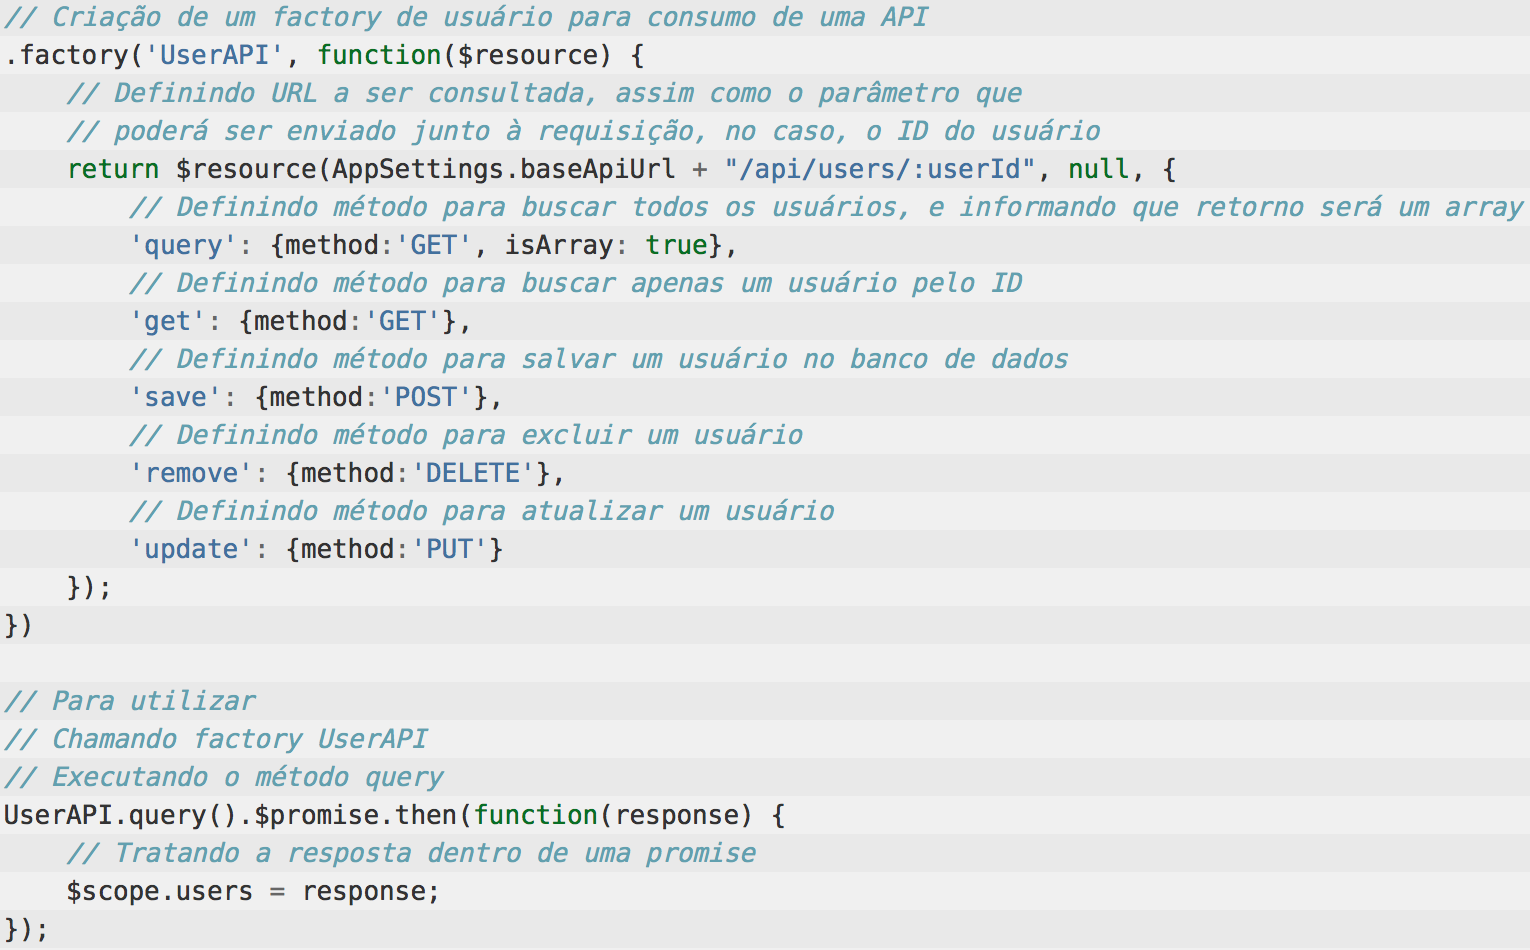
\includegraphics[width=1\textwidth]{codes/ionic/resource}
	\caption[Requisição utilizando o ngResource no Ionic]{Requisição utilizando o ngResource no Ionic. Baseado em Github\protect\footnotemark}
	\label{fig:resource-ionic}
\end{figure}
\begin{figure}[H]
	\centering
	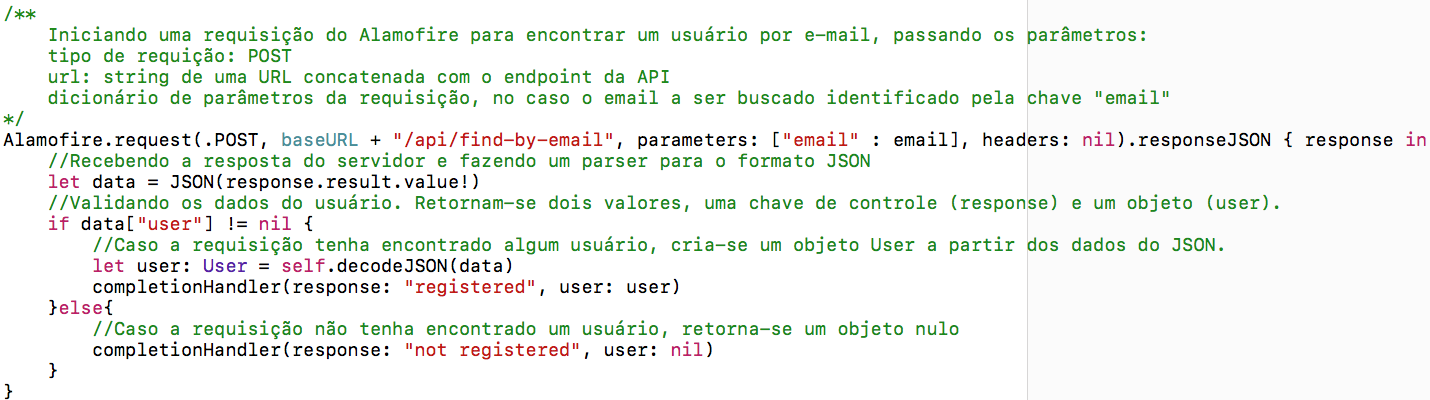
\includegraphics[width=1\textwidth]{codes/ios/alamofire}
	\caption[Requisição utilizando Alamofire e SwiftyJSON no iOS]{Requisição utilizando Alamofire e SwiftyJSON no iOS}
	\label{fig:alamofire-ios}
\end{figure} 
\begin{figure}[H]
	\centering
	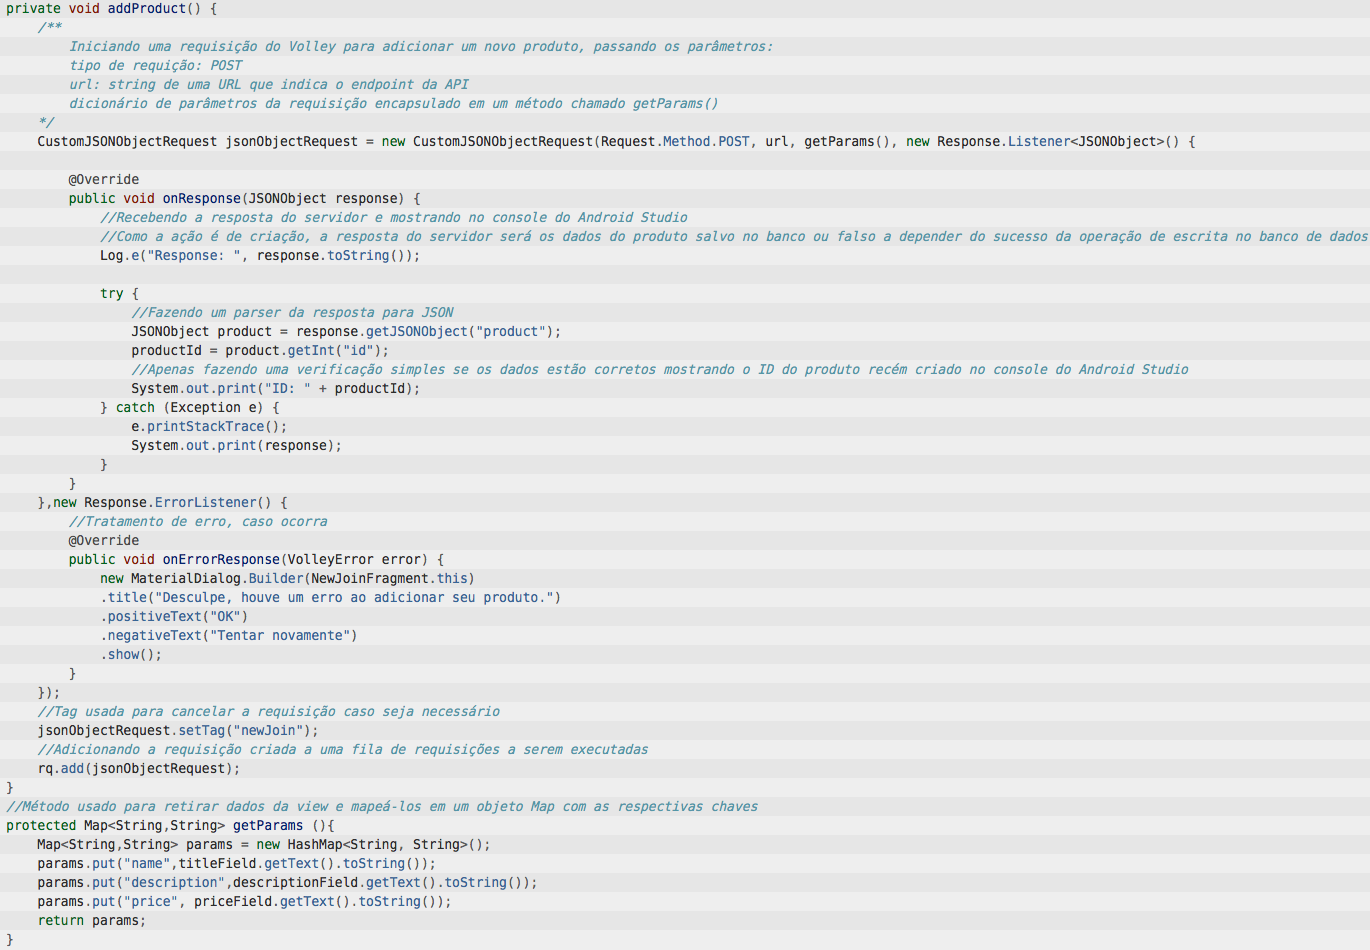
\includegraphics[width=1\textwidth]{codes/android/volley}
	\caption[Requisição utilizando Volley no Android]{Requisição utilizando Volley no Android}
	\label{fig:volley-android}
\end{figure}

\footnotetext{\url{https://github.com/fga-gpp-mds/2016.1-Partiu_frontend}}

\subsubsection{Extração de metadados de arquivos} \label{subsubsec:extracaometadata}
Em alguns casos, pode ser necessário a extração de metadados de algum arquivo específico, como uma imagem ou um áudio. No caso de uma imagem, podem ser retiradas informações como local, hora de criação e até mesmo 
dados climáticos no momento da captura da foto. No caso de um arquivo de áudio, é possível extrair o título do áudio, o autor ou artista, tempo de duração e álbum. Esses metadados podem ser usados para 
melhorar a experiência de uso do aplicativo fornecendo sugestões e funcionalidades mais próximas das necessidades reais do usuário, ou até mesmo para fazer filtros e buscas mais inteligentes nos dados que o 
aplicativo manuseia. 

Para extração de metadados no iOS existem classes nativas como a \textit{AVPlayerItem} e \textit{ALAssetsLibrary} para extração de metadados, respectivamente, de audio e imagens. No Android existe a 
classe \textit{MediaMetadataRetriever}, que lida com a extração de tipos variados de mídia. Em ambos os casos, iOS e Android, a implementação é simples, pois é preciso apenas seguir os métodos das classes 
utilizando constantes do sistema para indicar qual dado se deseja obter. Por exemplo, se o objetivo é obter a informação de título, no iOS, basta chamar pela \textit{string} ``title''. Já no Android, para o mesmo 
objetivo, basta chamar pela \textit{string} ``METADATA\_KEY\_TITLE''.

A seguir são apresentados trechos de códigos implementando a extração de metadados no iOS e no Android.

\begin{figure}[H]
	\centering
	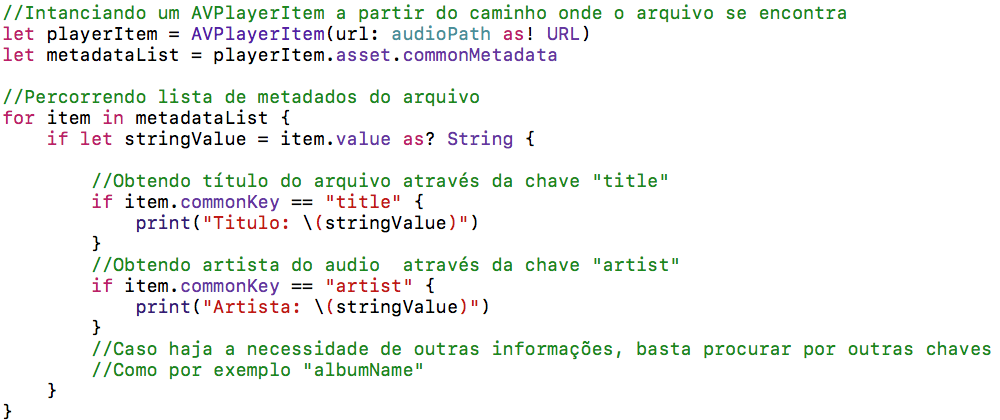
\includegraphics[width=1\textwidth]{codes/ios/metadata_audio}
	\caption[Extração de metadados de um arquivo áudio no iOS]{Extração de metadados de um arquivo áudio no iOS}
	\label{fig:metadata_audio-ios}
\end{figure}

\begin{figure}[H]
	\centering
	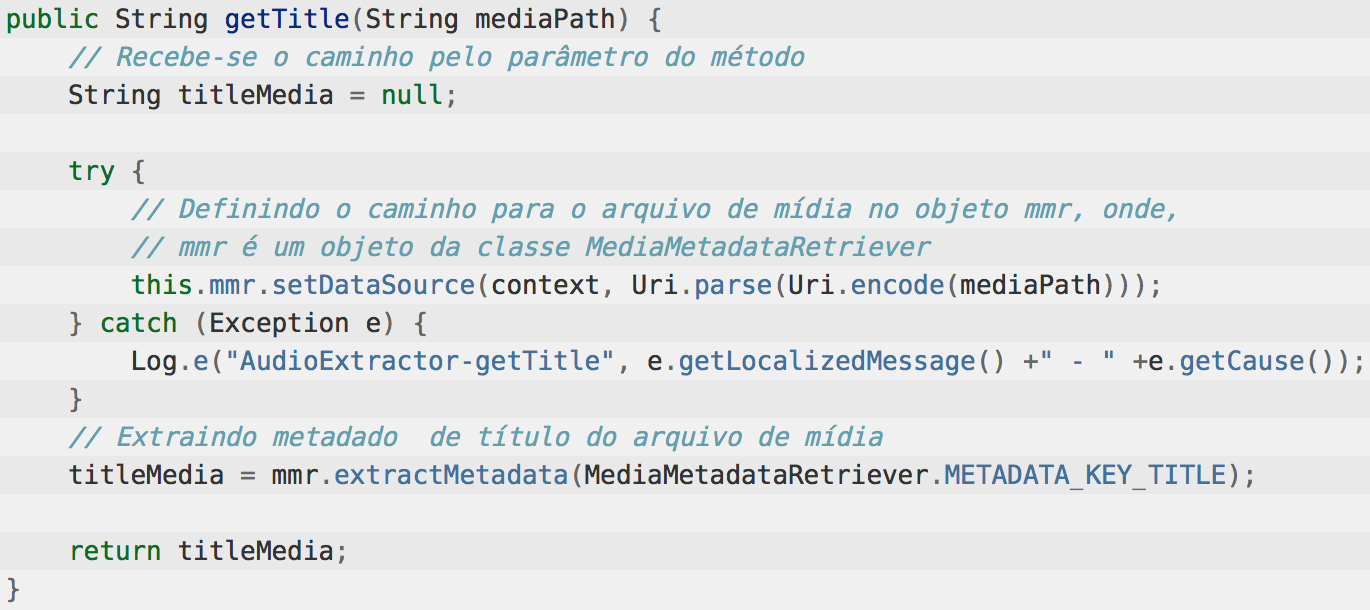
\includegraphics[width=1\textwidth]{codes/android/metadata_midia}
	\caption[Extração de metadados de um arquivo áudio no Android]{Extração de metadados de um arquivo áudio no Android. Baseado em Github\protect\footnotemark}
	\label{fig:metadata_midia-android}
\end{figure}

\footnotetext{\url{https://github.com/adorilson/MMUnB}}
%\begin{figure}[H]
%	\centering
%	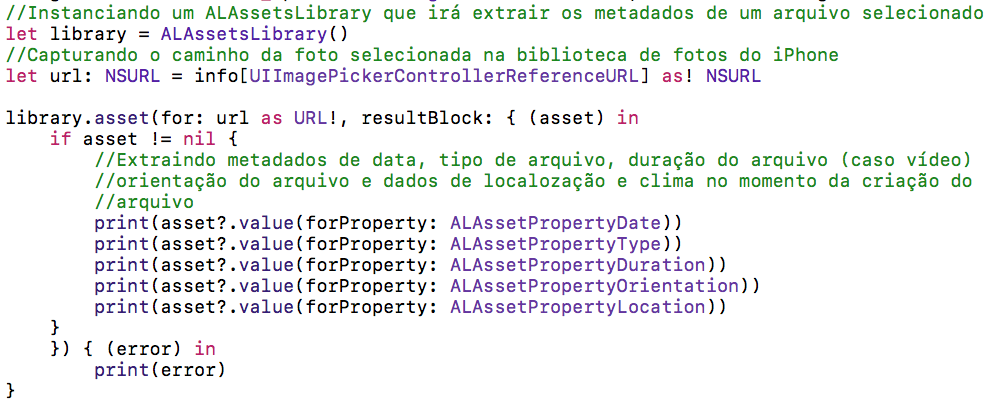
\includegraphics[width=1\textwidth]{codes/ios/metadata_video}
%	\caption[Trecho de código para extrair metadados de vídeo - iOS]{Trecho de código para extrair metadados de vídeo - iOS}
%	\label{fig:metadata_video-ios}
%\end{figure}

\textcolor{red}{... parecer sobre Ionic ...}

\subsubsection{Detecção de força do toque} \label{subsubsec:forcetouch}
Em 2015, alguns dispositivos móveis foram comercializados com uma tecnologia de detecção de pressão nas telas sensíveis ao toque. Primeiramente pela companhia chinesa Huawei e depois pela Apple, trata-se de um recurso 
capaz de identificar a quantidade de força que o usuário exerceu em um toque, o que abre o leque de possibilidades para novas funcionalidades nos aplicativos desenvolvidos. 
No iOS, é chamado de \textit{3DTouch} e por enquanto está disponível nos modelos de iPhone 6S ou superior. No Apple Watch e no novo MacBook, assim como no Mate S, da Huawei, é chamado apenas de \textit{Force Touch}, 
nome original da tecnologia. 
Vale ressaltar que o Android já possui a capacidade de ler a área de toque por meio de \textit{software} apenas, no entanto, o \textit{Force Touch} não é apenas a leitura de área de toque, mas sim da pressão do toque,
o que envolve \textit{hardware} e \textit{software}.

A seguir são apresentados trechos de código iOS e Ionic para utilização do \textit{3DTouch} criando \textit{Quick Actions}, uma funcionalidade do iOS que permite que o usuário aperte com mais força o ícone do aplicativo 
para ter algumas opções antes de entrar no aplicativo.

\begin{figure}[H]
	\centering
	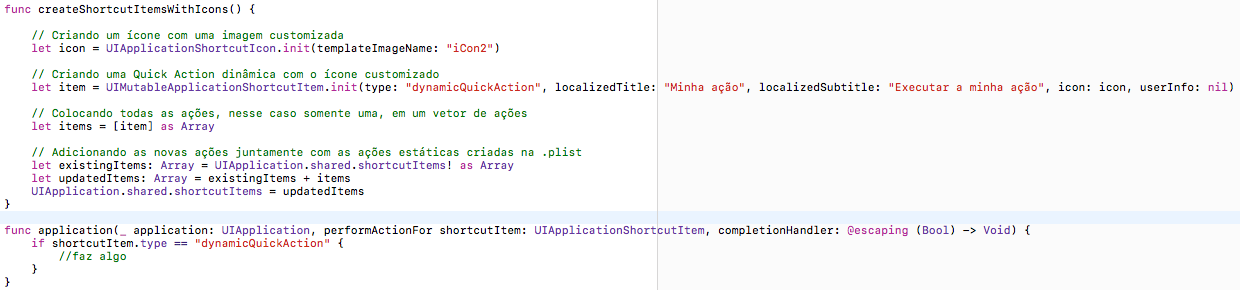
\includegraphics[width=1\textwidth]{codes/ios/3dtouch}
	\caption[Trecho de código implementando 3DTouch no iOS.]{Trecho de código implementando 3DTouch no iOS. Fonte: Baseado em Github\protect\footnotemark}
	\label{fig:3dtouch-ios}
\end{figure}

\footnotetext{\url{https://github.com/versluis/3D-Touch}}

\begin{figure}[H]
	\centering
	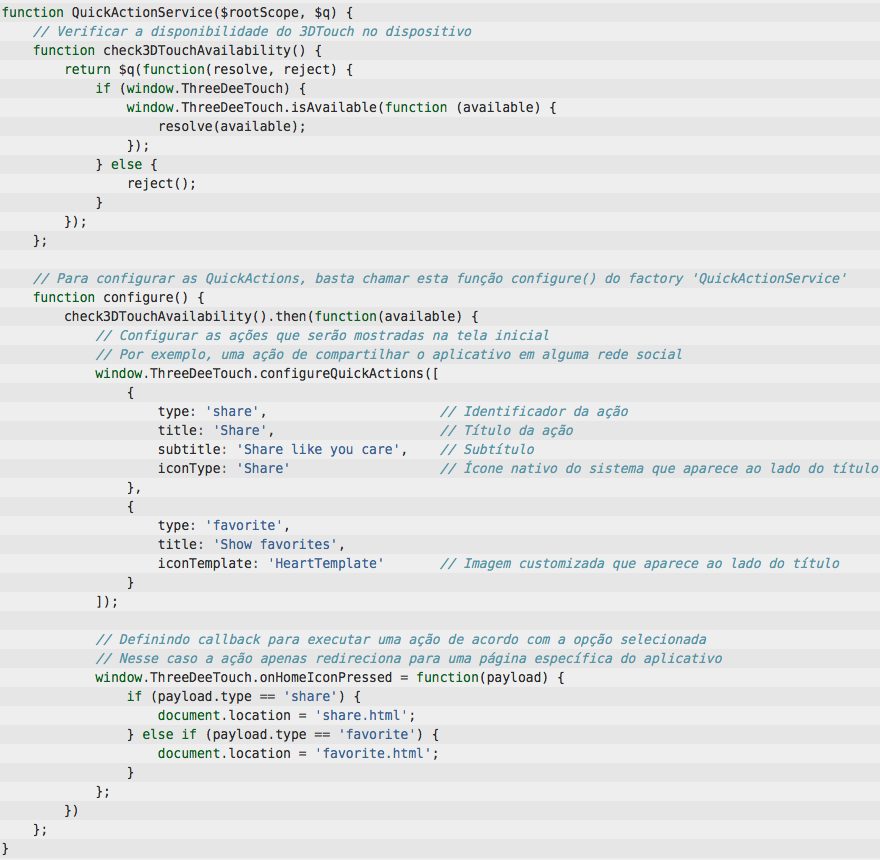
\includegraphics[width=1\textwidth]{codes/ionic/forcetouch}
	\caption[Trecho de código implementando 3DTouch no Ionic]{Trecho de código implementando 3DTouch no Ionic. Fonte: Baseado em Github\protect\footnotemark}
	\label{fig:forcetouch-ionic}
\end{figure}

\footnotetext{\url{https://github.com/ashteya/ionic-tutorial-quickactions}}

Em ambos os casos a implementação é simples apenas devendo-se considerar as diferenças entre plataformas e linguagens, no entanto, no caso do Ionic é necessária a utilização do 
\textit{plugin cordova-plugin-3dtouch}\footnote{\url{https://github.com/EddyVerbruggen/cordova-plugin-3dtouch}}.

\subsubsection{\textit{Smartwatches}} \label{subsubsec:facial} 

Além de \textit{smartphones} e \textit{tablets}, estão começando a ficar populares os dispositivos \textit{vestíveis} como relógios inteligentes. Isso implica em mais plataformas para dominar 
e mais possibilidades de aplicativos e funcionalidades para desenvolver. Um dos \textit{smartwatches} mais populares, atualmente, é o Apple Watch. Lançado com um sistema operacional próprio derivado do iOS, o WatchOS, 
por enquanto, funciona como uma extensão dos aplicativos criados para iPhone, ou seja, adiciona funcionalidades de rápida interação ao relógio para que não seja necessário interagir com o celular a todo momento.

Caso haja a necessidade de criar um aplicativo que suporte o Apple Watch, pode-se optar por desenvolver multiplataforma também, pois já existem \textit{plugins}
\footnote{\url{https://github.com/leecrossley/cordova-plugin-apple-watch}} 
do Cordova para realizar a integração entre o aplicativo multiplataforma e a extensão para Apple Watch. No entanto, o \textit{plugin} citado só funciona enquanto o aplicativo no iPhone está rodando. Quando, por algum motivo, 
o aplicativo deixa de rodar o \textit{plugin} não consegue mais se comunicar com o relógio podendo prejudicar a experiência de uso do aplicativo. Com isso, pode não ser uma boa ideia utilizar funcionalidades que 
precisam de atualização em tempo real, por exemplo, que recebe dados de um servidor, pois se o aplicativo no iPhone não estiver rodando, o relógio não conseguirá se comunicar e pegar os dados mais recentes, fazendo com 
que apresente dados desatualizados, prejudicando a experiência de uso.

Vale ressaltar que o aplicativo no Apple Watch deve ser feito nativamente, diretamente no Xcode! O \textit{plugin} apenas fornece um meio para que o \textit{app} multiplataforma do iPhone possa transmitir e receber dados do \textit{app}
do relógio, mas não é possível criar a interface e controladoras do relógio via multiplataforma, pois o Apple Watch não possui um navegador (\textit{WebView}) para interpretar o JavaScript assim como o iPhone. Então, 
deve ser feito o aplicativo utilizando Cordova e Ionic, por exemplo, para o iPhone, e depois criar o \textit{app} no Xcode para Apple Watch e então utilizar um \textit{plugin} para realizar a comunicação entre os dois aplicativos.  

Se o aplicativo planeja utilizar muitos recursos do Apple Watch, como frequencímetro, pedômetro e acelerômetro, como aplicativos voltados para a área da saúde por exemplo, pode ser melhor desenvolver nativamente,
pois o foco não estará sendo em desenvolver o aplicativo para várias plataformas, mas sim para um dispositivo específico. Com isso, pode-se aproveitar melhor todos os recursos do relógio e todos os benefícios da integração
do mesmo com o iPhone.

Caso o aplicativo já exista, ainda que seja multiplataforma, é possível desenvolver o aplicativo para o relógio, no entanto, a comunicação entre o iPhone e o relógio não será perfeita no multiplataforma como é no nativo, 
o que implica em limitar as funcionalidades do aplicativo no relógio para não prejudicar a experiência do usuário, podendo até mesmo fazer com que não valha a pena investir tempo e esforço na criação do aplicativo para
relógio. Cabe ressaltar que também já existem \textit{plugins}\footnote{\url{https://github.com/tgardner/cordova-androidwear}} do Cordova para Android Wear, os \textit{smartwatches} que rodam Android. 

\subsubsection{Envio de e-mail e SMS} \label{subsubsec:emailsms}


\subsubsection{\textit{Widgets}} \label{subsubsec:widgets}

\subsubsection{Siri} \label{subsubsec:siri}

\subsubsection{Acessibilidade} \label{subsubsec:acessibilidade}

\subsubsection{Touch ID} \label{subsubsec:touchid}

\subsubsection{Câmeras customizadas} \label{subsubsec:customcamera}

\subsubsection{Reconhecimento facial} \label{subsubsec:facial}
dizer que isso eh possivel nativamente usando tais e tais apis e multiplataforma usando adobe air
se quiser fazer em multiplataforma tbm eh possivel


\subsubsection{\textit{Smart TV}} \label{subsubsec:tv}
Assim como os \textit{smartwatches}, também existem outros dispositivos que estão ficando cada vez mais inteligentes e conectados à \textit{internet}, como por exemplo, os aparelhos de televisão. Alguns já vêm
com um sistema inteligente de fábrica, no entanto, é possível acoplar centrais multimídia ao televisor por meio de cabos \textit{HDMI} e à \textit{internet} por meio de \textit{Wi-fi} ou conexão \textit{ethernet}, 
deixando-os mais inteligentes e úteis. Alguns exemplos comerciais são a Apple TV, da Apple, e o Chrome Cast do Google. É possível desenvolver aplicativos para os televisores, aproveitando ao máximo os recursos de 
áudio e vídeo do aparelho, tornando a experiência com televisão ainda mais imersiva e prática. 

Cada plataforma possui sua própria \textit{SDK} para desenvolvimento dos aplicativos para TV e embora já existam \textit{plugins} do Cordova para lidar com o desenvolvimento de aplicativos para Apple TV e Chrome Cast, 
não há motivos suficientes para utilizá-los, pois o aplicativo criado não será portado para ambas as plataformas (iOS e Android) e para cada nova funcionalidade que cada TV desenvolver, deverá ser desenvolvido o 
\textit{plugin} para utilizá-la, ao passo que no desenvolvimento nativo, será possível utilizar o máximo de cada plataforma sempre, respeitando sempre os guias de usabilidade de cada uma. 

Caso a equipe de desenvolvimento já possua conhecimentos em \textit{HTML, CSS, JavaScript} e \textit{Cordova}, pode ser vantajoso desenvolver o aplicativo multiplataforma, considerando o tempo de densenvolvimento, por 
mais que tenha que ser feito em dois projetos distintos, um para iOS e um para Android, pois a \textit{expertise} da equipe pode compensar. No entanto, ainda será necessário possuir conta de desenvolvedor, um computador com 
MacOS e Xcode para subir o aplicativo iOS para a loja, por isso caso já haja alguém com experiência no ambiente e plataforma da Apple, desenvolver nativamente seria mais recomendado nas atuais circunstâncias. 

Assim como os \textit{smartwatches}, as TVs possuem guias de estilo e usabilidade muito diferentes dos dispositivos móveis, pois possuem tamanhos de telas e recursos de \textit{hardware} e \textit{software} completamente 
distintos, ou seja, o desenvolvimento multiplataforma está cada vez mais difícil por ter que, cada vez mais, abarcar um gama de dispositivos muitos diferentes, variando em tamanhos que vão de uma polegada e meia a
até mais de 100 polegadas e sistemas operacionais, com \textit{SDKs}, \textit{frameworks}, \textit{hardware} e recursos próprios de cada plataforma. 